%%
%% This is file `sample-acmsmall.tex',
%% generated with the docstrip utility.
%%
%% The original source files were:
%%
%% samples.dtx  (with options: `all,journal,bibtex,acmsmall')
%%
%% IMPORTANT NOTICE:
%%
%% For the copyright see the source file.
%%
%% Any modified versions of this file must be renamed
%% with new filenames distinct from sample-acmsmall.tex.
%%
%% For distribution of the original source see the terms
%% for copying and modification in the file samples.dtx.
%%
%% This generated file may be distributed as long as the
%% original source files, as listed above, are part of the
%% same distribution. (The sources need not necessarily be
%% in the same archive or directory.)
%%
%%
%% Commands for TeXCount
%TC:macro \cite [option:text,text]
%TC:macro \citep [option:text,text]
%TC:macro \citet [option:text,text]
%TC:envir table 0 1
%TC:envir table* 0 1
%TC:envir tabular [ignore] word
%TC:envir displaymath 0 word
%TC:envir math 0 word
%TC:envir comment 0 0
%%
%% The first command in your LaTeX source must be the \documentclass
%% command.
%%
%% For submission and review of your manuscript please change the
%% command to \documentclass[manuscript, screen, review]{acmart}.
%%
%% When submitting camera ready or to TAPS, please change the command
%% to \documentclass[sigconf]{acmart} or whichever template is required
%% for your publication.
%%
%%
% \documentclass[acmsmall]{acmart}
% \documentclass[manuscript]{acmart}
\documentclass[acmsmall,screen]{acmart}

\usepackage{amsmath,amsfonts}
\usepackage{algorithm}
% \usepackage{algorithmic}
\usepackage{array}
\usepackage[caption=false,font=normalsize,labelfont=sf,textfont=sf]{subfig}
\usepackage{textcomp}
\usepackage{stfloats}
\usepackage{url}
\usepackage{verbatim}
\usepackage{graphicx}
\usepackage{hyperref}
\usepackage{textcomp}
\usepackage{xcolor}
\usepackage{tabularx}
\usepackage{listings}
\usepackage{multirow}
\usepackage{enumitem}
% \usepackage{hyperref}
\usepackage{pifont}
\usepackage[breakable]{tcolorbox}
\usepackage{adjustbox}
\usepackage{booktabs}
\usepackage[flushleft]{threeparttable}
\usepackage[noend]{algpseudocode}

\usepackage{xurl}
\def\UrlBreaks{%
	\do\/%
	\do\a\do\b\do\c\do\d\do\e\do\f\do\g\do\h\do\i\do\j\do\k\do\l%
	\do\m\do\n\do\o\do\p\do\q\do\r\do\s\do\t\do\u\do\v\do\w\do\x\do\y\do\z%
	\do\A\do\B\do\C\do\D\do\E\do\F\do\G\do\H\do\I\do\J\do\K\do\L%
	\do\M\do\N\do\O\do\P\do\Q\do\R\do\S\do\T\do\U\do\V\do\W\do\X\do\Y\do\Z%
	\do0\do1\do2\do3\do4\do5\do6\do7\do8\do9\do=\do/\do.\do:%
	\do\*\do\-\do\~\do\'\do\"\do\-}
\urlstyle{same}

% Define custom colors
\definecolor{mylinkcolor}{RGB}{0, 0, 0} % Black color for links
\definecolor{mycitecolor}{RGB}{128, 0, 128} % Purple color for citation links
\definecolor{mycitebg}{RGB}{173, 216, 230} % Light blue color for citation background

% Set up hyperref with custom colors
\hypersetup{
	colorlinks=true,         % false: boxed links; true: colored links
	linkcolor=mylinkcolor,   % color of internal links (change box color with linkbordercolor)
	citecolor=mycitecolor,   % color of citation links
	urlcolor=mylinkcolor,    % color of external links
	linkbordercolor=mycitebg % background color for citation links
}

\definecolor{verylightgray}{rgb}{.97,.97,.97}
\lstdefinelanguage{Solidity}{
	keywords=[1]{anonymous, assembly, assert, balance, break, call, callcode, case, catch, class, constant, continue, constructor, contract, debugger, default, delegatecall, delete, do, else, emit, event, experimental, export, external, false, finally, for, function, gas, if, implements, import, in, indexed, instanceof, interface, internal, is, length, library, log0, log1, log2, log3, log4, memory, modifier, new, payable, pragma, private, protected, public, pure, push, require, return, returns, revert, selfdestruct, send, solidity, storage, struct, suicide, super, switch, then, this, throw, transfer, true, try, typeof, using, value, view, while, with, addmod, ecrecover, keccak256, mulmod, ripemd160, sha256, sha3}, % generic keywords including crypto operations
	keywordstyle=[1]\color{blue}\bfseries,
	keywords=[2]{address, bool, byte, bytes, bytes1, bytes2, bytes3, bytes4, bytes5, bytes6, bytes7, bytes8, bytes9, bytes10, bytes11, bytes12, bytes13, bytes14, bytes15, bytes16, bytes17, bytes18, bytes19, bytes20, bytes21, bytes22, bytes23, bytes24, bytes25, bytes26, bytes27, bytes28, bytes29, bytes30, bytes31, bytes32, enum, int, int8, int16, int24, int32, int40, int48, int56, int64, int72, int80, int88, int96, int104, int112, int120, int128, int136, int144, int152, int160, int168, int176, int184, int192, int200, int208, int216, int224, int232, int240, int248, int256, mapping, string, uint, uint8, uint16, uint24, uint32, uint40, uint48, uint56, uint64, uint72, uint80, uint88, uint96, uint104, uint112, uint120, uint128, uint136, uint144, uint152, uint160, uint168, uint176, uint184, uint192, uint200, uint208, uint216, uint224, uint232, uint240, uint248, uint256, var, void, ether, finney, szabo, wei, days, hours, minutes, seconds, weeks, years},	% types; money and time units
	keywordstyle=[2]\color{teal}\bfseries,
	keywords=[3]{block, blockhash, coinbase, difficulty, gaslimit, number, timestamp, msg, gas, sender, sig, value, now, tx, gasprice, origin},	% environment variables
	keywordstyle=[3]\color{violet}\bfseries,
	keywords=[4]{mload,create,create2,add},
	keywordstyle=[4]\color{red}\bfseries,
	identifierstyle=\color{black},
	sensitive=true,
	comment=[l]{//},
	morecomment=[s]{/*}{*/},
	commentstyle=\color{gray}\ttfamily,
	stringstyle=\color{red}\ttfamily,
	morestring=[b]',
	morestring=[b]",
}

% 定义代码块样式
\lstdefinestyle{codestyle}{
	language=Solidity, % 选择代码块的语言
	basicstyle=\ttfamily\scriptsize, % 设置基本样式,如字体、大小等
	keywordstyle=\color{blue}, % 设置关键字的样式
	commentstyle=\color{green!60!black}, % 设置注释的样式
	stringstyle=\color{red}, % 设置字符串的样式
	breaklines=true, % 允许代码块自动换行
	numbers=left, % 在左侧显示行号
	numberstyle=\tiny\color{black}, % 设置行号的样式
	stepnumber=1, % 设置行号递增的步长
	frame=single, % 设置代码块的边框
	xleftmargin=15pt, % 设置行号左侧的距离
% backgroundcolor=\color{gray!5}, % 设置代码块的背景颜色
	captionpos=b, % 设置标题位置为底部
}
\lstset{style=codestyle}


\newtcolorbox{answerbox}{
	colback=gray!12, % 背景颜色
	colframe=white,  % 边框颜色
	arc=4pt,         % 圆角半径
	boxrule=0pt,     % 边框宽度
	left=6pt,        % 左边距
	right=6pt,       % 右边距
	boxsep=0pt,      % 文本框和内容之间的间距
	breakable,
}

% Define custom colors
\definecolor{mylinkcolor}{RGB}{0, 0, 0} % Black color for links
\definecolor{mycitecolor}{RGB}{128, 0, 128} % Purple color for citation links
\definecolor{mycitebg}{RGB}{173, 216, 230} % Light blue color for citation background

%%
%% \BibTeX command to typeset BibTeX logo in the docs
\AtBeginDocument{%
	\providecommand\BibTeX{{%
		Bib\TeX}}}

%% Rights management information.  This information is sent to you
%% when you complete the rights form.  These commands have SAMPLE
%% values in them; it is your responsibility as an author to replace
%% the commands and values with those provided to you when you
%% complete the rights form.
\setcopyright{acmlicensed}
\copyrightyear{2025}
\acmYear{2025}
\acmDOI{XXXXXXX.XXXXXXX}

%%
%% These commands are for a JOURNAL article.
% \acmJournal{JACM}
% \acmVolume{37}
% \acmNumber{4}
% \acmArticle{111}
% \acmMonth{8}

%%
%% Submission ID.
%% Use this when submitting an article to a sponsored event. You'll
%% receive a unique submission ID from the organizers
%% of the event, and this ID should be used as the parameter to this command.
%%\acmSubmissionID{123-A56-BU3}

%%
%% For managing citations, it is recommended to use bibliography
%% files in BibTeX format.
%%
%% You can then either use BibTeX with the ACM-Reference-Format style,
%% or BibLaTeX with the acmnumeric or acmauthoryear sytles, that include
%% support for advanced citation of software artefact from the
%% biblatex-software package, also separately available on CTAN.
%%
%% Look at the sample-*-biblatex.tex files for templates showcasing
%% the biblatex styles.
%%

%%
%% The majority of ACM publications use numbered citations and
%% references.  The command \citestyle{authoryear} switches to the
%% "author year" style.
%%
%% If you are preparing content for an event
%% sponsored by ACM SIGGRAPH, you must use the "author year" style of
%% citations and references.
%% Uncommenting
%% the next command will enable that style.
%%\citestyle{acmauthoryear}


%%
%% end of the preamble, start of the body of the document source.
\begin{document}

%%
%% The "title" command has an optional parameter,
%% allowing the author to define a "short title" to be used in page headers.
	\title[Investigating and Understanding Factory-related Smart Contracts]{Investigating and Understanding Factory-related Smart Contracts: Prevalence, Implementation, and Security Issues}

%%
%% The "author" command and its associated commands are used to define
%% the authors and their affiliations.
%% Of note is the shared affiliation of the first two authors, and the
%% "authornote" and "authornotemark" commands
%% used to denote shared contribution to the research.
	\author{Ziyue Wang}
	\email{ziyue0530@gmail.com}
	\orcid{0009-0000-6621-4712}


	\author{ZongWen Shen}
	\email{szw@smail.nju.edu.cn}
	\orcid{0009-0005-2492-2530}


	\author{Lei Chen}
	\email{willisgarey89@gmail.com}
	\orcid{0009-0000-9079-3427}
	\affiliation{%
		\institution{National Key Laboratory for Novel Software Technology, Nanjing University}
		\city{Nanjing}
		\state{Jangsu}
		\country{China}
	}

	\author{Wei Song}
	\email{wsong@njust.edu.cn}
	\orcid{0000-0002-4324-3382}
	\affiliation{%
		\institution{Nanjing University of Science and Technology}
		\city{Nanjing}
		\state{Jangsu}
		\country{China}
	}

	\author{Jidong Ge}
	\email{gjd@nju.edu.cn}
	\orcid{0000-0003-1773-0942}
	\authornote{Corresponding Authors.}
	\affiliation{%
		\institution{National Key Laboratory for Novel Software Technology, Nanjing University}
		\city{Nanjing}
		\state{Jangsu}
		\country{China}
	}

	\author{LiGuo Huang}
	\email{lghuang@lyle.smu.edu}
	\orcid{0000-0001-7790-0195}
	\affiliation{%
		\institution{Department of Computer Science, Southern Methodist University}
		\city{Dallas}
		\state{Texas}
		\country{USA}}

	\author{Bin Luo}
	\email{luobin@nju.edu.cn}
	\orcid{0000-0002-9036-0063}
	\affiliation{%
		\institution{National Key Laboratory for Novel Software Technology, Nanjing University}
		\city{Nanjing}
		\state{Jangsu}
		\country{China}
	}


%%
%% By default, the full list of authors will be used in the page
%% headers. Often, this list is too long, and will overlap
%% other information printed in the page headers. This command allows
%% the author to define a more concise list
%% of authors' names for this purpose.
	\renewcommand{\shortauthors}{Trovato et al.}

%%
%% The abstract is a short summary of the work to be presented in the
%% article.
	\begin{abstract}
		As the demand for creating and deploying diverse decentralized applications increases, smart contract factories have become essential infrastructure. These contracts offer a convenient mechanism to automate the deployment of smart contracts. Currently, implementation patterns based on factories are proliferating, and security considerations related to \underline{F}actory-related \underline{S}mart \underline{C}ontracts (FSCs) should be systematically investigated. The unique context and diverse implementation patterns of FSCs call for an in-depth understanding from developers; otherwise, security issues may be introduced. However, existing works only focus on singular aspects of FSCs, lacking a comprehensive investigation of implementation patterns related to factory-related smart contracts, as well as a thorough detection and analysis of FSC security issues.

		Our study aims to uncover the current state of practice and security issues of FSCs. To achieve this goal, we first develop a static detector to collect factory contracts and factory-deployed contracts. Then we conduct a large-scale empirical analysis on 482,542 Ethereum contracts to address the questions regarding FSC prevalence, FSC implementation and FSC security issues. Our findings reveal that factory contracts dominate in contract deployment, with an average of 92.7\% of Ethereum contracts deployed by factories. FSCs have found primary applications across four key domains of smart contracts, including finance, NFT, decentralized infrastructure, and proxy. Moreover, our research summarizes six factory-based implementation patterns and discovers a total of 1,180 real-world FSC security issues involving four categories. We further explore their safety implications, providing security guidance for smart contract development practices.
	\end{abstract}

%%
%% The code below is generated by the tool at http://dl.acm.org/ccs.cfm.
%% Please copy and paste the code instead of the example below.
%%
	\begin{CCSXML}
		<ccs2012>
		<concept>
		<concept_id>10002978.10003006.10003013</concept_id>
		<concept_desc>Security and privacy~Distributed systems security</concept_desc>
		<concept_significance>500</concept_significance>
		</concept>
		</ccs2012>
	\end{CCSXML}

	\ccsdesc[500]{Security and privacy~Distributed systems security}

%%
%% Keywords. The author(s) should pick words that accurately describe
%% the work being presented. Separate the keywords with commas.
	\keywords{Solidity, smart contract factory, factory pattern, security analysis.}

% \received{20 February 2007}
% \received[revised]{12 March 2009}
% \received[accepted]{5 June 2009}

%%
%% This command processes the author and affiliation and title
%% information and builds the first part of the formatted document.
	\maketitle

	\section{Introduction}\label{sec:intro}
	Smart contracts \cite{smartcontract} are blockchain programs widely used in decentralized finance (DeFi) and the Internet of Things (IoT), forming key Web3 infrastructure. As one of the most prominent blockchain platforms, Ethereum, \cite{ethereum} supports smart contract deployment and development, hosting over 66 million Solidity contracts as of January 2025 \cite{smart_contract_deployment}.

	In recent years, the rise of complex decentralized applications (DApps) has made contract deployment and management crucial \cite{DBLP:journals/ese/ChenXLGY21,DBLP:conf/wcre/TsiounisK22,DBLP:journals/tse/ZouLKLXFCX21,DBLP:conf/IEEEcloud/NayakNSK18}. However, manually writing and deploying contracts is repetitive and risky, rendering it unsuitable for dealing with the demand of large-scale contract deployment. To address this, developers are increasingly deploying contracts with the help of smart contract factories \cite{factory-contract} as advocated by Ethereum improvement proposals (EIPs) \cite{eip-1014,eip-1167,eip-2470,eip-3171} and third-party libraries \cite{openz-clones,0age-metamorphic,openz-create2,openz-proxyfactory,nft-factory}. This factory manner ensures efficient and scalable deployment, and provides solutions to critical concerns such as contract upgradeability and gas optimization. In our study, these factories and factory-deployed contracts are collectively referred to as \textbf{Factory-related Smart Contracts (FSCs)}.

	With the widespread applications of FSCs, some security risks have raised concerns \cite{eip-2470,create2-security-discussion,tornado-cash-attack,tornado-cash-attack2}. On the one hand, developers are required to have a deep understanding of the implementation of FSCs to avoid issues like those highlighted by EIP-2470 (Singleton Factory) \cite{eip-2470}. The proposal underscores that contracts deployed by a factory should avoid using \textit{msg.sender} in the constructor to specify ownership, as failure to comply this may lead to access control problems. On the other hand, despite intense discussions within the Ethereum community \cite{create2-security-discussion} regarding potential FSCs security issues, these contracts can be used by attackers as a tool to carry out malicious activities \cite{tornado-cash-attack,tornado-cash-attack2,op-stolen}. As reported in May 2023, the attack on the Tornado Cash governance community in May 2023 \cite{tornado-cash-attack2} serves as a stark reminder of the challenge that comes with FSC security issues. It marks the first utilization of metamorphic contract technology. Specifically, the attack is initiated with a specially crafted governance proposal that is modified under the same address to allow theft of funds just after it is approved. This incident ultimately results in a loss of 3.2 million US dollars \cite{tornado-cash-attack}. Furthermore, a survey \cite{twitter-survey} shows 76\% of contract developers and auditors lack an understanding of relevant security issues.

	However, existing studies have two main research gaps. \textbf{(1) Insufficient consideration of security issues within the FSC context.} Many studies focus on detecting general smart contract security issues \cite{DBLP:conf/pldi/BrentGLSS20,DBLP:conf/kbse/XueMLSYP20,DBLP:conf/issta/GhalebRP22,DBLP:conf/issta/LiaoZCN22,DBLP:conf/uss/0001L21}, discussing traditional vulnerabilities like reentrancy. To the best of our knowledge, no work considers to detect specific security issues within the context of factory smart contracts (FSCs). For example, the Tornado Cash DAO attack involves a dynamic process of factory contract deployment, contract self-destruction, and contract redeployment. Detecting this vulnerability requires tools to be able to: determine the deployer account type; distinguish create/create2 deployment methods; identify critical operations (\textit{selfdestruct} / \textit{delegatecall} / \textit{callcode}). Although the mentioned analyzers can effectively detect the \textit{selfdestruct} / \textit{delegatecall} operations, they cannot retrieve or assess the contract deployer or account type. Additionally, existing work has never considered the risks associated with the \textit{create} / \textit{create2} instructions.
	\textbf{(2) Lack of a comprehensive investigation of factories and factory-deployed contracts.} While some empirical studies explore FSC characteristics \cite{DBLP:conf/sigsoft/SunXLLL23,DBLP:conf/fc/FrowisB22,DBLP:conf/fc/SalehiCM22,DBLP:journals/pacmpl/ChaliasosGL22}, for example, Chaliasos et al. investigate the prevalence of \textit{create} / \textit{create2} opcodes in Solidity inline assembly blocks \cite{DBLP:journals/pacmpl/ChaliasosGL22}. However, they only cover a singular dimension and lack comprehensive real-world investigations into FSCs, limiting smart contract developers’ thorough understanding. The aforementioned attack and the survey demonstrate how insufficient understanding of the smart contracts lifecycle can lead to overlooked vulnerabilities. This gap is not merely theoretical but has significant real-world consequences.


	To bridge the two gaps, we undertake a large-scale empirical study on Ethereum FSCs, with the aim of answering the following research questions. \textbf{RQ1:} How prevalent are FSCs? \textbf{RQ2:} What are unique functionalities and factory-based implementation patterns of FSCs? \textbf{RQ3:} Are there undisclosed security issues in FSCs, and what impacts do they pose? The answers to these questions are valuable for Ethereum community security and smart contract deployment. For instance, Solidity developers can benefit from our findings to decide whether to use a factory for deployment. They can also develop a fully functional factory contract with safety design considerations. In addition, many studies are dedicated to reducing the gas cost in deploying contracts \cite{DBLP:conf/kbse/Li21a,DBLP:journals/jss/SorboLVVC22,DBLP:journals/tosem/AlbertGHRS22}. Our study, detailed in Section~\ref{sec:4.3}, elucidates a gas optimization pattern provided by factories. Furthermore, developers can utilize our proposed four FSC security detectors to detect metamorphic contracts and other issues. Finally, the Ethereum community can gain insights through our security case studies, aiding in the formulation of preventive measures.

	To address the above research questions, we gather 482,542 contracts deployed on the Ethereum mainnet. Then we develop a FSC detector to extract factory and factory-deployed contracts. We proceed to quantify their prevalence and categorize the application domains. We further explore the implementation patterns and security risks in FSCs development and governance. Through a deeper understanding of FSCs, we also provide practical countermeasures to mitigate security threats.

	Our key findings include: \ding{172} FSCs dominate smart contract deployment, with over 90\% of contracts on the Ethereum mainnet from 2020 to 2024 deployed by factories;  create2-based factories account for 49.8\% post-constantinople upgrade. \ding{173} FSCs find primary applications in Finance, NFT, Decentralized Infrastructure, and Proxy, driving further development and innovation within Ethereum's ecosystem. \ding{174} Among the six factory-based patterns identified, the Template Configuration Pattern and Proxy Delegation Pattern stand out as the most prevalent. These patterns underscore the benefits of factory contracts in deploying multiple contract instances with identical bytecode. \ding{175} Despite constituting only 0.72\% of Ethereum factory contracts, the metamorphic pattern poses significant security risks, necessitating comprehensive security audits across the entire contract deployment chain. \ding{176} We identify a total of 1,180 real-world FSCs with security issues, involving four categories: \textit{Mutable Code}, \textit{Unexpected Ownership Transfer}, \textit{Unhandled Low-Level Contract Creation}, and \textit{Unverified Master Contract}. In summary, this paper makes the following contributions:
	\begin{itemize}[leftmargin=0.4cm,topsep=0.1cm]
		\item We conduct a comprehensive empirical study on FSCs with 482,542 smart contracts from Ethereum mainnet, covering contract names, code, and transactions.
		\item We design and implement a FSC detector along with four security checkers, each targeting a specific security issue related to FSCs that we have newly discovered.
		\item We gain many novel insights into FSCs from three dimensions, enriching the comprehension of FSC development and security issues.
		\item To facilitate community and future research, we make all our research artifacts publicly available at \url{https://anonymous.4open.science/r/FSCs-empirical-analysis}.
	\end{itemize}

	The rest of paper is organized as follows. We first introduce background in Section~\ref{sec:background}. Then we detail methodology and present findings in Section~\ref{sec:methodology} and Section~\ref{sec:findings}, respectively. We further delve into discussion in Section~\ref{sec:discussions}, summarize related work in Section~\ref{sec:relatedwork}, and conclude in Section~\ref{sec:conclusion}.


	\section{Background Knowledge}\label{sec:background}
	In this section, we introduce the background knowledge that is useful for understanding our research.

	\subsection{Smart Contracts}
	Smart contracts \cite{smartcontract} are self-executing contracts with the terms of the agreement directly written into code. These contracts are designed to automatically enforce and execute pre-defined rules and conditions, eliminating the need for trusted intermediaries and fostering transparency in transactions. While various smart contract programming languages exist, Solidity \cite{solidity} is the predominant language used for developing smart contracts on Ethereum and other Ethereum Virtual Machine (EVM)-compatible blockchains.
	A Solidity smart contract comprises several key components, including:
	\begin{itemize}[leftmargin=0.4cm,topsep=0.1cm]
		\item State Variables: These variables store the contract's persistent data, representing its current state. They hold information such as account balances, ownership records, and configuration parameters.
		\item Functions: Functions define the contract's behavior and logic. They are executable units of code that can be called by external users or other smart contracts to interact with the contract's state.
		\item Modifiers: Modifiers are code blocks that can be attached to functions to enforce pre-conditions. They provide a mechanism for access control, validation, and other security checks before a function can be executed. For example, a common modifier is onlyOwner, which restricts function execution to the contract owner.
		\item Events: Events allow smart contracts to log actions and state changes that occur during execution. These logs can be monitored by external applications to track contract activity and trigger off-chain processes.
	\end{itemize}

	\subsection{Ethereum and Etherscan}


	Ethereum \cite{ethereum} represents a significant advancement in blockchain technology, serving as a pioneering public, permissionless, and distributed computing platform. While building upon the foundational principles established by Bitcoin \cite{Bitcoin}, Ethereum expands the application of blockchain beyond a purely peer-to-peer digital currency system. It achieves this by enabling the deployment and execution of smart contracts, programmable agreements that automatically execute when predefined conditions are met. This capability has unlocked a new paradigm for decentralized applications (dApps) across a wide range of industries.

	At the heart of Ethereum lies the Ethereum Virtual Machine (EVM) \cite{EVM}, a Turing-complete runtime environment that executes the bytecode of smart contracts. The EVM provides a deterministic and isolated execution environment, ensuring that contracts behave predictably and securely, regardless of the underlying hardware. The EVM's architecture is crucial for maintaining the integrity and consistency of the Ethereum blockchain. Gas \cite{Gas}, a unit of computation, is used to measure the computational cost of executing operations on the EVM, preventing denial-of-service attacks and ensuring fair resource allocation.

	Etherscan \cite{etherscan} is a prominent blockchain explorer and analytics platform specifically designed for the Ethereum network. It provides a user-friendly interface for accessing and analyzing data stored on the Ethereum blockchain, including transactions, smart contracts, addresses, and blocks. Etherscan's functionalities are essential for developers, researchers, and users seeking to understand the workings of the Ethereum ecosystem. Key features of Etherscan include:
	\begin{itemize}
		\item Transaction Tracking: Users can track the status and details of individual transactions, including sender, recipient, gas used, and transaction fee.
		\item Smart Contract Inspection: Etherscan allows users to view the source code of verified smart contracts, enhancing transparency and enabling security audits.
		\item Address Analysis: Users can analyze the transaction history and balance of specific Ethereum addresses, gaining insights into their activity on the network.
	\end{itemize}


	\subsection{Factory-related Smart Contracts}
	Smart contract factories \cite{factory-contract} have emerged as a critical component of decentralized infrastructure, streamlining the creation and deployment of smart contracts. These factory contracts offer a programmatic means to deploy new contract instances, automating the process and enabling scalable deployment of decentralized applications. Prominent examples include the UniswapV2Factory used by the Uniswap \cite{uniswap} decentralized exchange to deploy UniswapV2Pair contracts for each trading pair, and the ERC20Factory contract offered by platforms like ThirdWeb \cite{thirdweb}, which allows users to rapidly generate new ERC-20 tokens with minimal coding effort. For terminological brevity, we refer to factory contract and factory-deployed contracts collectively as \underline{F}actory-related \underline{S}mart \underline{C}ontracts (FSCs) in our study.
% 更清晰的解释这个定义,以免再被审稿人误解


	\begin{figure}[h]
		\centering
		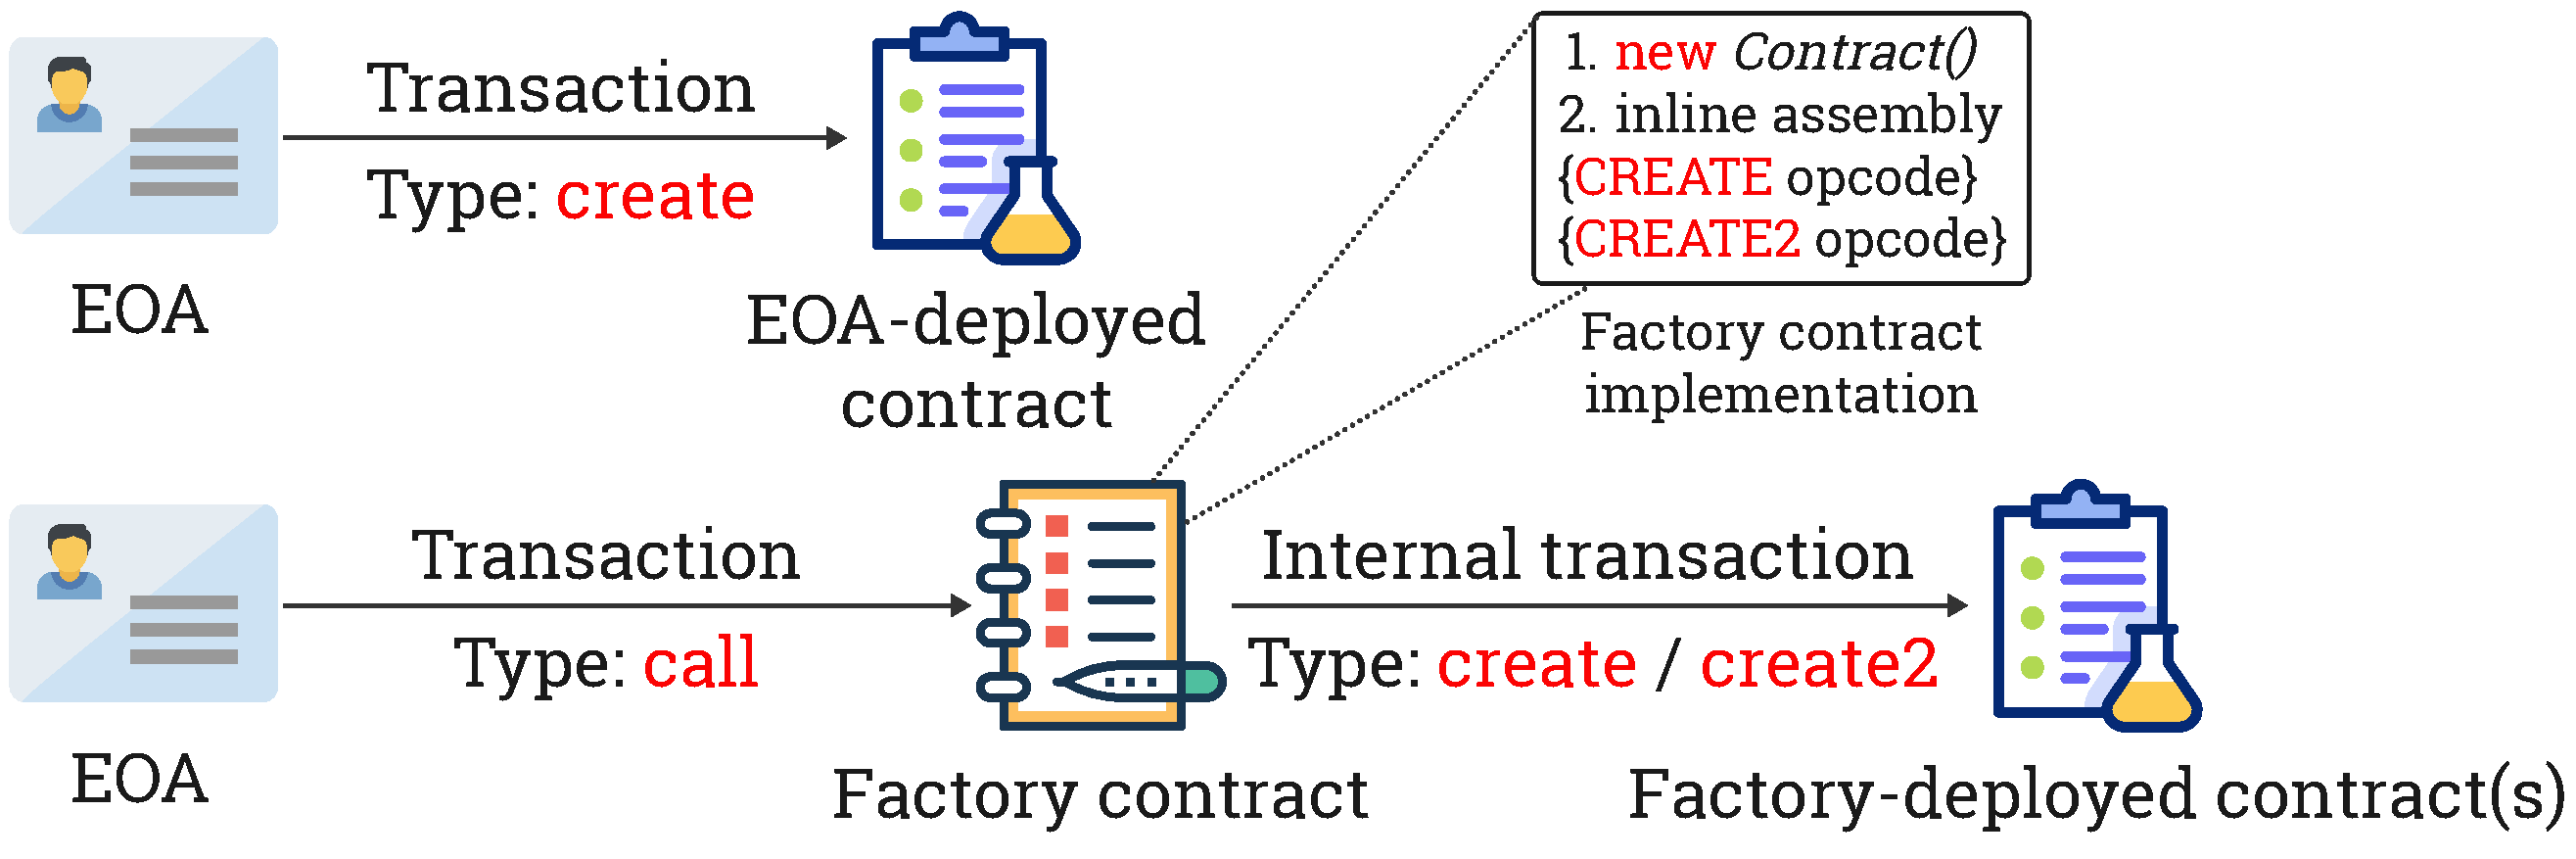
\includegraphics[width=0.6\linewidth]{figures/factoryvseoa.pdf}
		\caption{Two smart contract deployment methods: direct deployment from external accounts or deployment through factory contracts.}
		\label{fig:deployment}
	\end{figure}

	Figure~\ref{fig:deployment} illustrates the comparison between contracts deployed by \underline{E}xternally \underline{O}wned \underline{A}ccounts (EOA) \cite{ETHAccount} and those deployed through a factory contract. In a direct EOA deployment, an EOA initiates a create transaction, directly deploying a new contract to the blockchain. Conversely, factory deployment involves a two-stage process. First, an EOA sends a transaction to the factory contract, invoking a specific method designed to handle contract deployment. This transaction includes necessary parameters such as constructor arguments for the new contract, Ether (ETH) for initialization, and potentially a salt value, depending on the deployment method. The factory contract then initiates an internal transaction, using either the \textit{create} or \textit{create2} opcode, to execute the actual contract creation and deployment.


	The underlying mechanism of smart contract factories relies on two core EVM opcodes: \textit{create} and \textit{create2}. The \textit{create} opcode determines the deployment address using the formula \textit{addr = keccak256(rlp(sender, nonce))}, where sender represents the address of the account (in this case, the factory contract) creating the new contract, and nonce is the number of transactions sent by that account. This approach results in deployment addresses that are dependent on the factory's transaction history. The \textit{create2} opcode, introduced through EIP-1014 \cite{eip-1014}, offers a deterministic and more predictable deployment address calculation: \textit{addr = keccak256(0xff, sender, salt, keccak256(init\_code))}. Here, sender is the address of the factory contract, salt is a user-defined value (allowing for deterministic deployment), and \textit{init\_code} is the initialization code of the contract being deployed. Developers can trigger contract creation using the high-level \textit{new Contract()} statement within Solidity, which typically compiles to the \textit{create} opcode. Alternatively, developers can directly use these opcodes within inline assembly blocks for finer-grained control over the deployment process.


	\section{Study Methodology}\label{sec:methodology}
	In this section, we first provide a detailed explanation of the three research questions posed in Section~\ref{sec:intro}. Subsequently, we elaborate on the methodology adopted in our empirical study.
	\subsection{Research Questions}
	Our study aims to address three research questions.

	RQ1:\textbf{ FSC Prevalence}. We quantify the prevalence of FSCs in Ethereum. The results will serve as the foundation for subsequent research. \textit{How prevalent are factories in real-world contracts? What are the trends in factory contract deployment using create / create2 opcodes? What are the major application domains of FSCs?}

	RQ2: \textbf{FSC Functionalities and Patterns}. We delve into the technical details and implementation to provide a comprehensive development guide of FSCs. \textit{What unique functionalities do contract factories possess? What are the design patterns based on contract factories?}

	RQ3: \textbf{FSC Security Risks and Countermeasures}. We explore the security challenges of FSCs in the real world. \textit{What are the key security vulnerabilities to be aware of? How can these vulnerabilities be detected? What are their potential impacts? And how can these risks be mitigated or resolved?}

	\begin{figure}[t]
		\centering
		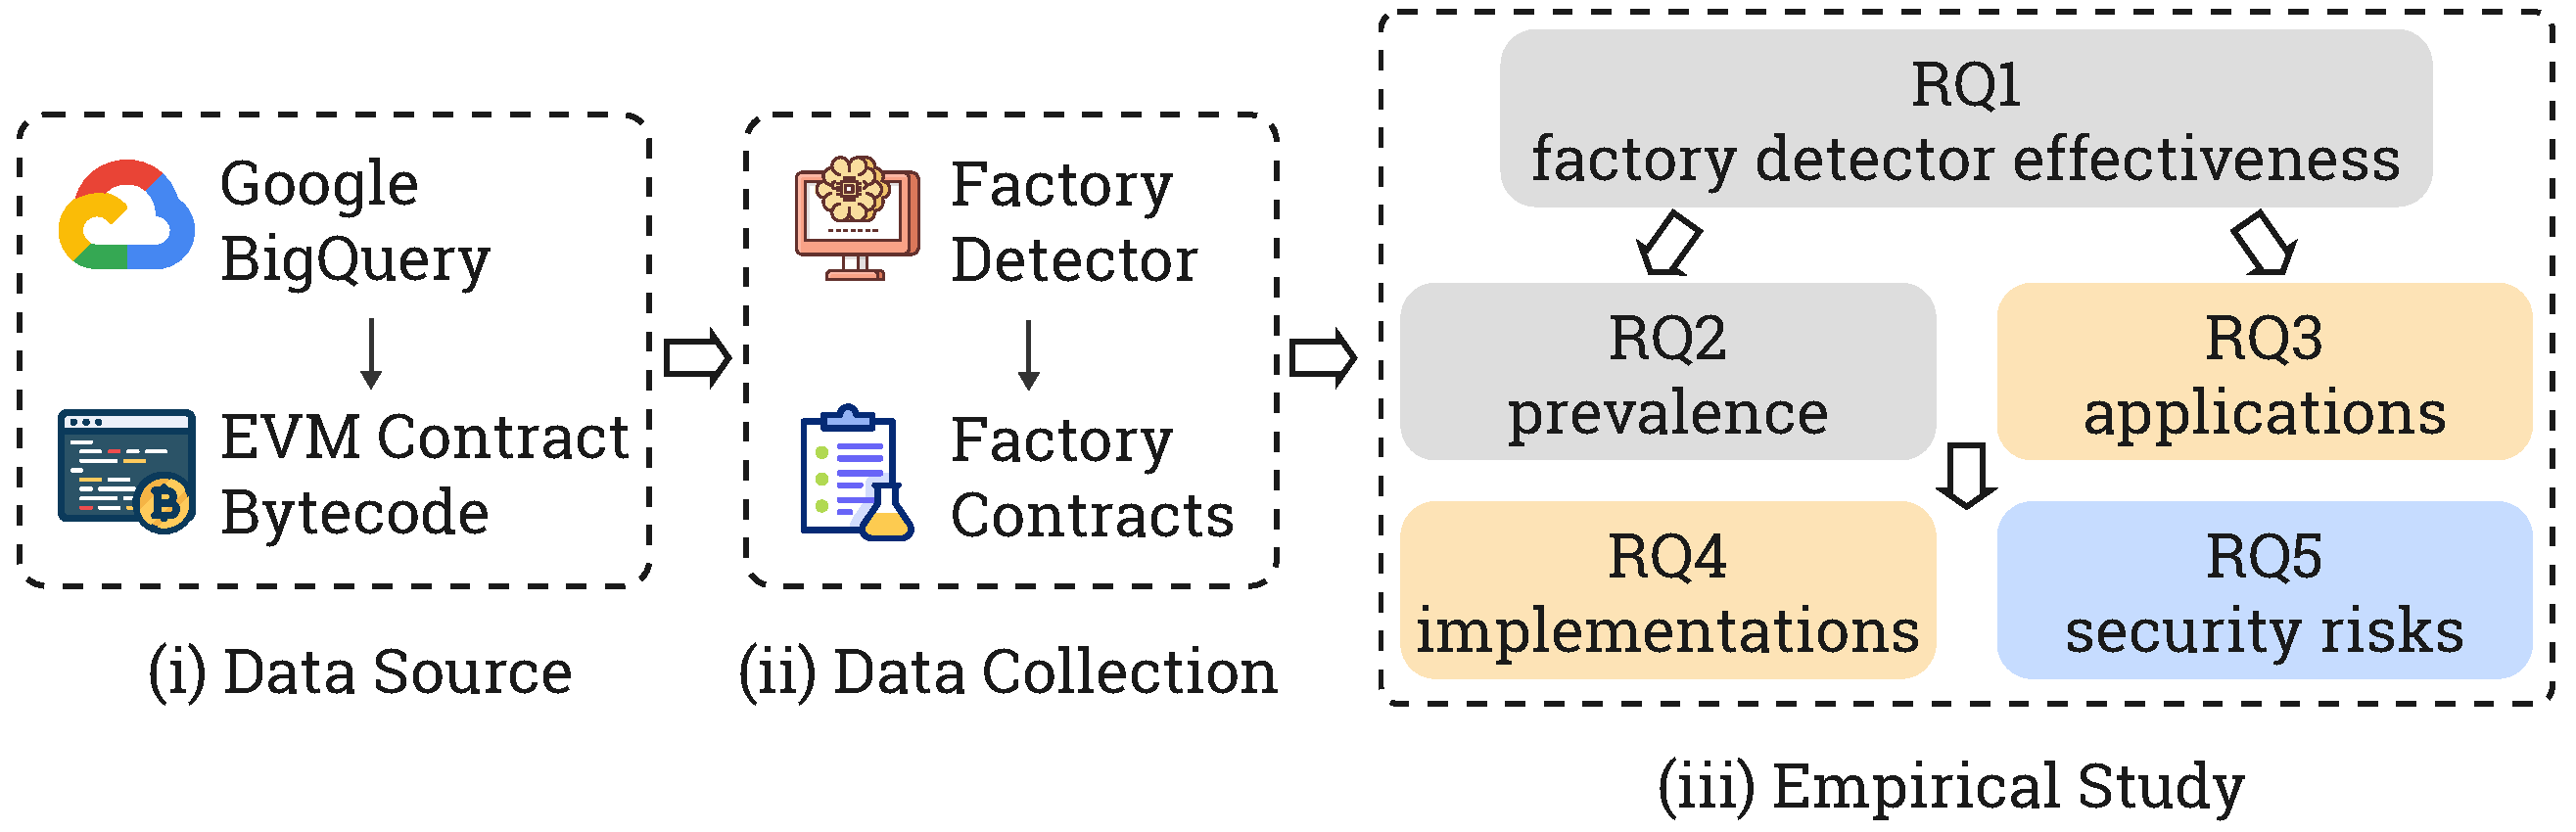
\includegraphics[width=0.85\linewidth]{figures/overview.pdf}
		\caption{The overall workflow of the study consists of five main steps: (1) Origin dataset collection; (2) Contract deployment chain construction and FSC dataset collection; (3) RQ1: prevalence and application domains analysis; (4) RQ2: functionalities and patterns analysis; (5) RQ3: security issues detection.}
		\label{fig:workflow}
	\end{figure}


	\subsection{Empirical Study Overview}
	As shown in Figure~\ref{fig:workflow}, we use GitHub open-source dataset \cite{opensourcedata} and Etherscan \cite{etherscan} to store Ethereum contracts. We detect factory contracts by using our factory detector, then query each factory’s deployer account and deployed contracts to construct deployment chains, forming our FSC dataset. Based on this dataset, we conduct the empirical study to address the three research questions.

	We leverage multiple tools for our study. The industry-leading smart contract analysis framework, Slither \cite{slither-tool} (version 0.9.6), is utilized to compile source code into IR and model the control flow. Solc-select \cite{solc-select} is used to automate switching between Solidity versions. Next, we will describe each step in detail.


% dataset collection
	\subsection{Origin Dataset Collection}
	We first use a widely used open-source smart contract dataset \cite{opensourcedata} to obtain 482,542 verified smart contract addresses deployed on the Ethereum mainnet. These contracts were deployed between 2017 and 2024. Next, we leverage the blockchain explorer Etherscan \cite{etherscan} to collect the source code for these contracts.


	\subsection{Contract Deployment Chain Construction and FSC Dataset Collection} Next, in order to further collect factory contracts and factory-deployed contracts based on the origin dataset, we need to address three key issues: (1) Identifying factory contracts; (2) Obtaining the deployer of the current contract and determining whether it is a contract account; (3) Collecting the contracts deployed by the factory contract. We implement the \textit{factory contract detector} to address issue (1), and we also implement a \textit{contract deployment chain constructor} to address issues (2) and (3). We describe the implementation of these two detectors and the FSC dataset in the following.

	\newcolumntype{R}{>{\raggedleft\arraybackslash}X} % Define the "R" column type
\begin{table}[t]
	\centering
	\footnotesize
	\caption{Dataset Overview}
	\label{tab:dataset}
	\begin{tabularx}
		{0.6\linewidth}{@{}lRR@{}} \toprule \textbf{Chain} & \textbf{Total Contract} & \textbf{Unique
		Bytecode} \\ \midrule Ethereum & 73,390,233 & 1,672,444 \\ Polygon & 361,151,932 & 2,008,503
		\\ Total & 434,542,165 & 3,680,947 \\ \bottomrule
	\end{tabularx}
\end{table}


	\subsubsection{Factory Contract Detector}
	Our FSC detector identifies factory contracts using the following two schemes: For verified contract with public source code, the detector utilizes Slither \cite{slither-tool} to query and compile the source code into IR. It then checks each function’s IR for \textit{new Contract()}, \textit{create}, or \textit{create2} opcodes. Based on this method, the detector can accurately determine the factory contract and does not introduce false positives. The left side of Figure~\ref{fig:chain} shows an example of the factory contract detection. For unverified contracts, we attempt to retrieve the bytecode and disassemble it to detect create or create2 opcodes. However, through experimentation, we find that current disassemblers, such as evmdasm \cite{evmdasm}, do not accurately translate bytecode into EVM instructions. For instance, the BeaconProxy \cite{BeaconProxy} contract’s source code does not contain \textit{create} or \textit{create2} assembly codes or \textit{new Contract()} statements. Yet, its deployed bytecode, when disassembled, incorrectly shows a \textit{create2} opcode. Therefore, This method leads to false positives and can impact the validity of subsequent experiments. Consequently, the detector detects factory contracts based on on-chain transactions. Initially, the detector retrieves the internal transactions using Etherscan, which provides detailed records of function calls. It further checks if there are multiple transaction records with the \textit{create} or \textit{create2} type. If so, it suggests that the contract includes functions for deploying new contracts, thus identifying the contract as a factory.

	\subsubsection{Contract Deployment Chain Constructor}\label{sec:deployment}
	Given the contracts in the origin dataset, beyond determining whether a contract is a factory contract, we also need to further determine the deployer of the contract and the contracts deployed by that contract. To systematically understand the deployment relationships between contracts, we propose the Contract Deployment Chain. For instance, if an \textit{EOA} deploys \textit{C1}, and \textit{C1} then deploys \textit{C2}, it forms a contract deployment chain: \textit{E → C1 → C2}.

	\begin{figure}[t]
		\centering
		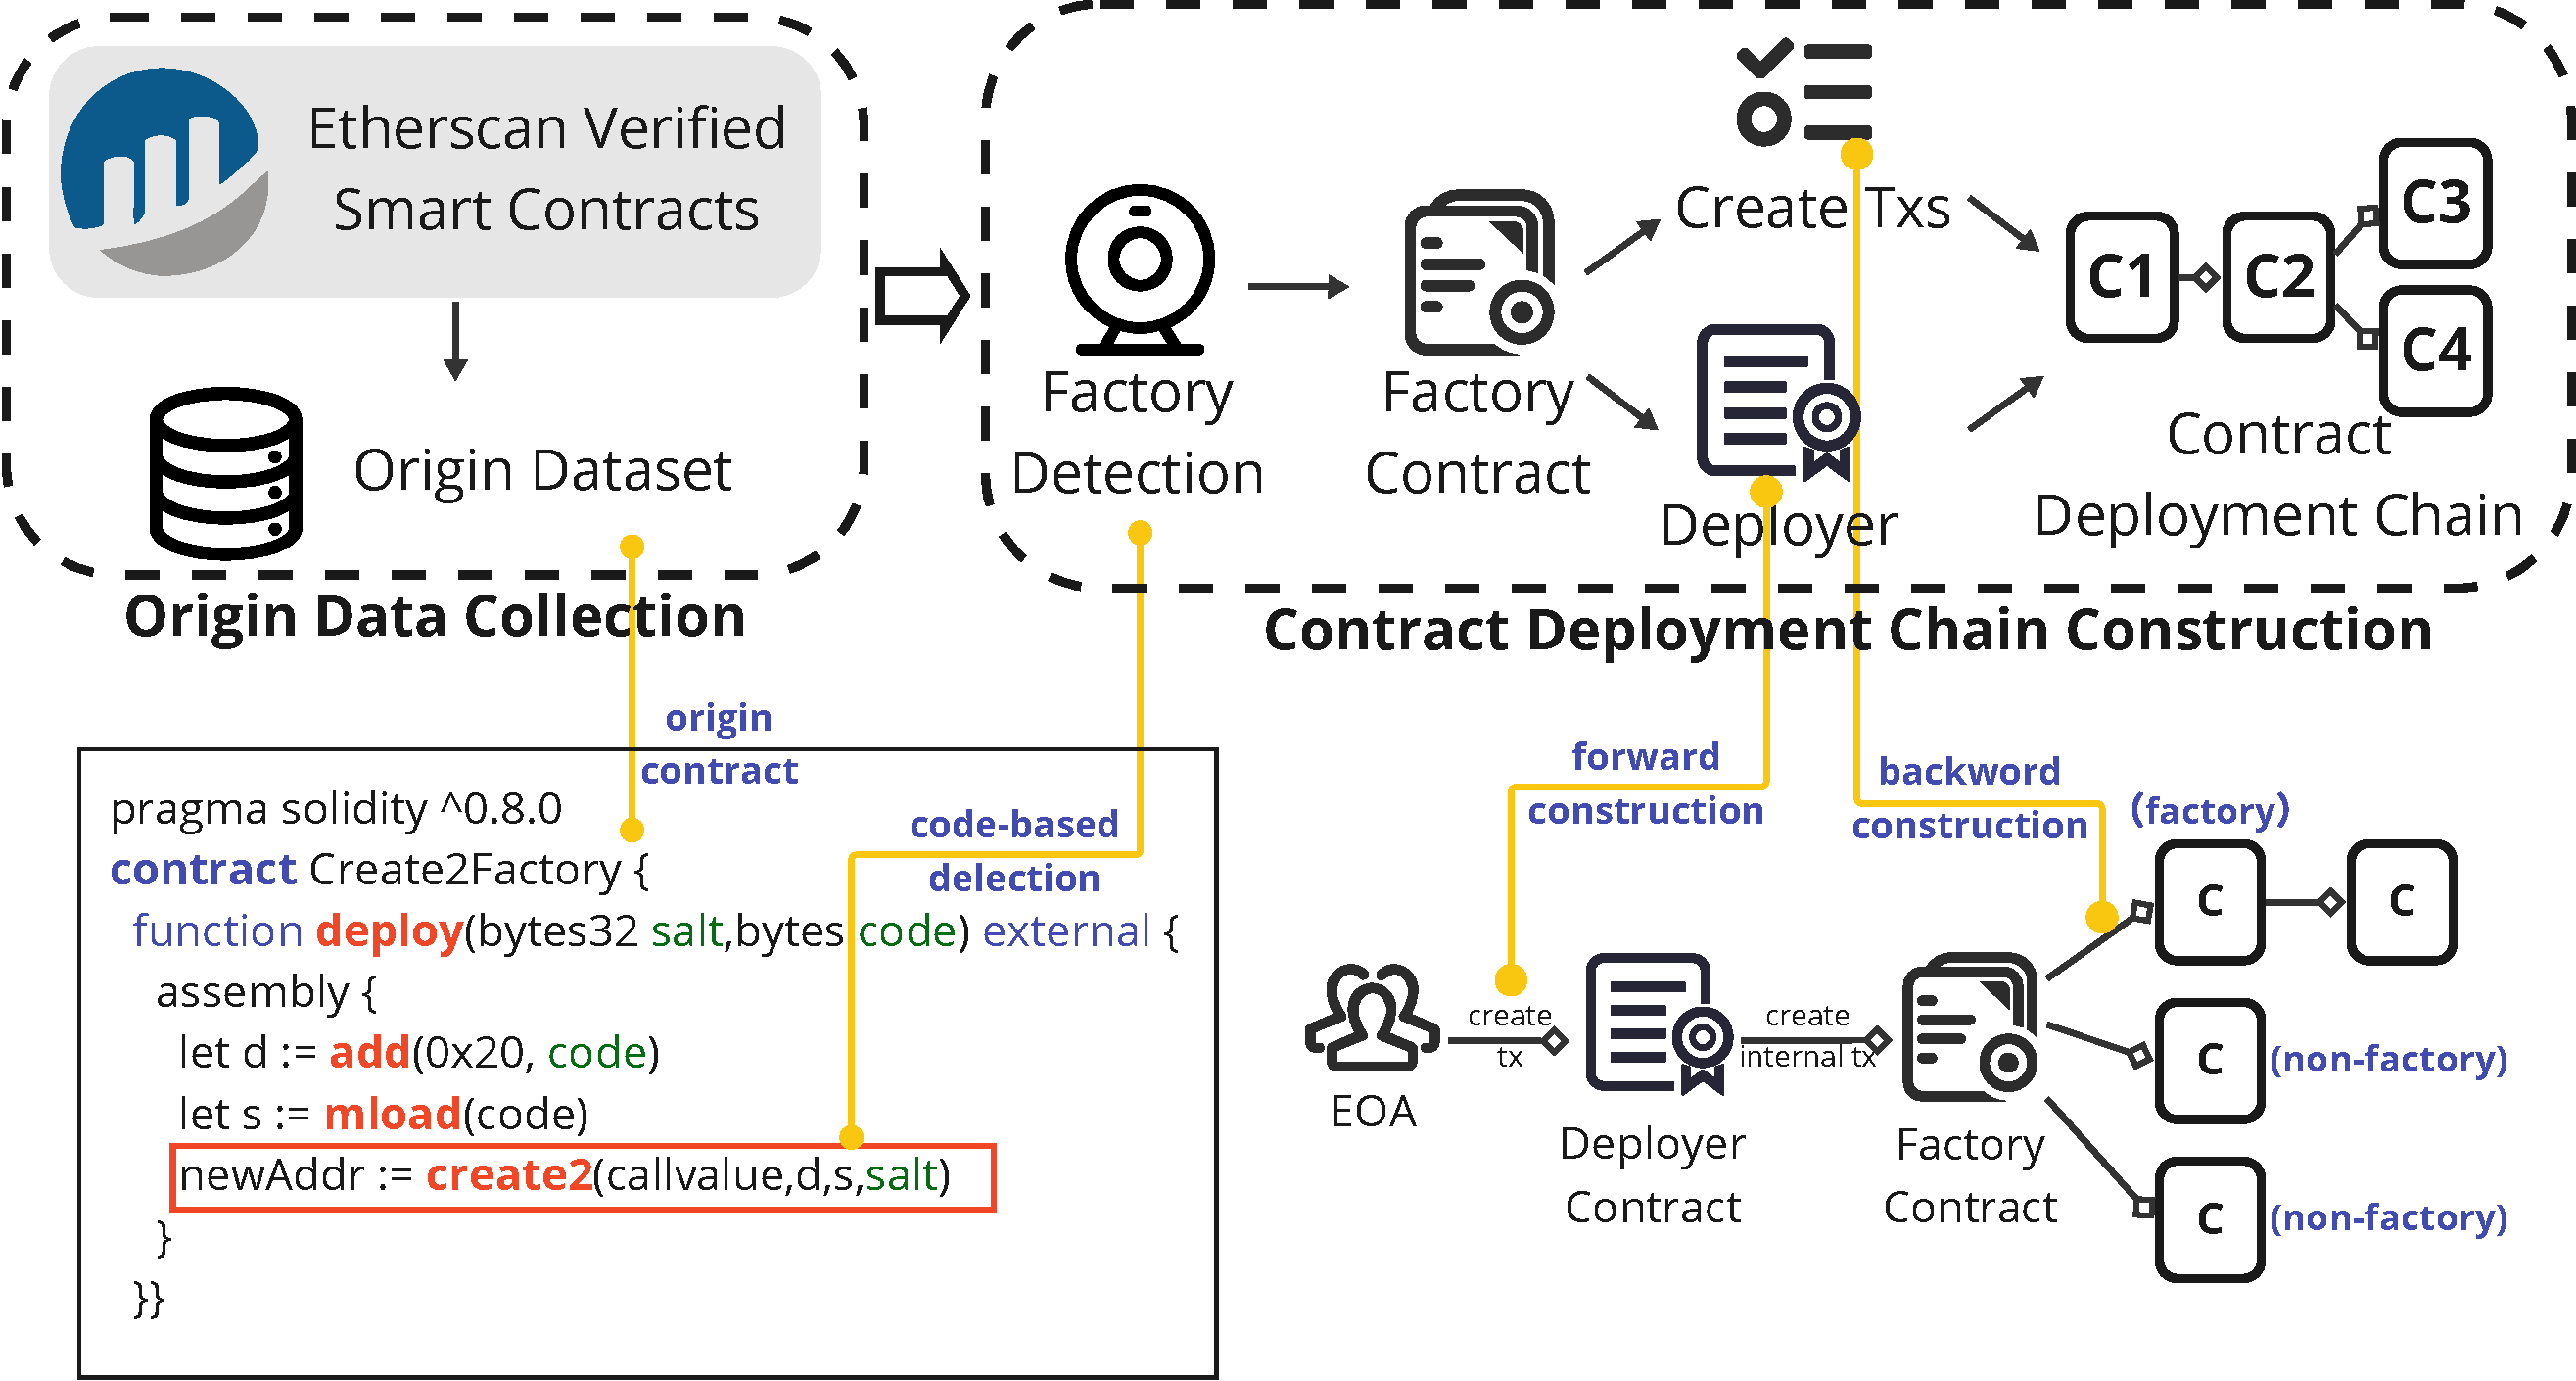
\includegraphics[width=0.85\linewidth]{figures/chain.pdf}
		\caption{The procedure of factory detection and contract deployment chain construction.}
		\label{fig:chain}
	\end{figure}

	The right side of Figure~\ref{fig:chain} illustrates the complete process of constructing a contract deployment chain given a contract. Specifically, the \textit{delpoyment chain constructor} constructs the contract deployment chain in two steps. \ding{172} Forward construction. Using the txhash of the transaction that creates the factory, it queries Etherscan for transaction info, checking if another factory has implemented it. If so, it repeats this process until the deployer's address corresponds to an external account.
	\ding{173} Backward construction. Using the factory contract address, it queries Etherscan for all internal \textit{create} or \textit{create2} transactions of the given contract, gathers all factory-deployed contracts, and links each factory with every contract it deploys. An example of a complete contract deployment chain is available in our public repository \cite{fscdata}.


	\subsubsection{FSC Dataset} We iterate through each contract in the origin dataset. First, we use the \textit{factory contract detector} to determine whether the contract is a factory. If it is, then we use the \textit{deployment chain constructor} to further construct the deployment chain and collect the factory contract and factory-deployed contracts within it. We ultimately identified and collected 8,083 factory contracts and 243,938 factory-deployed contracts with unique bytecode on the Ethereum mainnet. Each record contains five attributes: \ding{172} name, \ding{173} transactions, \ding{174} creation time, \ding{175} compiler version, \ding{176} source code if verified.


	\subsection{Prevalence Investigation (RQ1)}
	To quantify the prevalence of FSCs, we conduct experiments in three aspects: \ding{172} Factory contract quantity. To understand the fluctuations in the number of factories, we quantify their daily deployments on the Ethereum mainnet. Additionally, we examine the specific deployment methods (high-level / low-level) and types (\textit{create} / \textit{create2}) used by each factory. \ding{173} Factory-deployed contract tendency. To gain insights into the changing trends of contract deployment methods, we compare the daily number of contracts deployed by external accounts with those deployed by factories. We also calculate the proportion of factory-deployed contracts out of the total deployed contracts. In order to accurately track the changes in Ethereum contract data over time, experiments \ding{172} and \ding{173} utilize the professional blockchain analysis platform Dune \cite{dunedashboard} to obtain contract data based on two established query rules. \ding{174} FSC application domains. We conduct a clustering analysis of the dataset accumulated from our initial data gathering. The specific steps involved converting contract names into vector embeddings using Word2Vec \cite{DBLP:journals/corr/word2vec}, capturing semantic associations with clustering algorithms, and manually reviewing the clustering results by identifying the constructs incorporating EIP protocol name as part of their names.


	\subsection{Functionalities and Patterns Analysis (RQ2)}
	After exploring the prevalence of FSCs, our research delves into their behaviors and factory-based patterns. The major challenge is how to exhaustively and reliably enumerate functionalities and implementation patterns. Admittedly, analyzing all of the collected smart contract factories individually is non-trivial due to the significant manpower and time costs involved. To address this challenge, we prioritize verified factory contracts with high transaction volume to ensure that our analysis reflects the most representative behaviors and real-world usage patterns. Then we select the top 500 factory contracts. To ensure the reliability of our analysis, we engage three experts with experience in smart contract security auditing to assist in the investigation of FSCs. We require each auditor to analyze the contracts independently and hold weekly group discussions to minimize subjective bias.

	Specifically, we follow these three steps to uncover functionalities and implementation patterns of FSCs:
	\ding{172} Factory Decomposition.
	We obtain five main components of smart contracts from Solidity official documentation (version 0.8.23) \cite{soliditydoc}, including: \textit{State Variables}, \textit{Functions}, \textit{Modifiers},\textit{ Events}, \textit{Errors}. Our audit team manually review each contract, discuss them in groups, and enumerate their functionalities, ensuring that each functionality is based on a real-world implementation and correlate with multiple contract components. \ding{173} Factory-based Pattern Identification.
	After understanding factory behaviors, we explore factory-based patterns by examining contract semantics, motivations, and functionalities. We source Ethereum Improvement Proposals and Ethereum Requests for Comment related to FSCs. To minimize subjective judgments and disagreements, we adopt the approach of independent auditing by each member and regular expert meetings. \ding{174} Pattern Extraction.\label{sec:patternextra} After determining the type of all patterns, we use static analysis to detect each pattern in the dataset based on syntactic and semantic features. For instance, EIP-1167 \cite{eip-1167} introduces the Minimal Proxy or Clone Factory pattern, implemented by OpenZeppelin’s Clones library \cite{openz-clones}. We apply two predefined rules to identify its use. For OpenZeppelin implementation: we check for library imports and clone/cloneDeterministic calls. For custom implementation: we locate the \textit{create} / \textit{create} opcode, search for master address identifiers, extract proxy bytecode, and check for \textit{delegatecall} opcode.

	\subsection{Security Issues Detection (RQ3)}
	Similar to the challenges in RQ2, we need to comprehensively identify FSC-related security issues. Notably, since no tools currently support the detection of these issues, it is also challenging to implement a set of static analysis tools for automated detection. To address the first challenge, we focus on implementation differences among functionally similar contracts when exploring RQ2, uncovering potential security risks from code audits. Eventually, besides known metamorphic contract issues, we identify three new security risks in coding practices.
	Then, we implement four static detectors at the source code level, each addressing specific security issues: the \textit{Mutable Code Detector}, \textit{Ownership Transfer Detector}, \textit{Unhandled Low-Level Contract Creation Detector}, and \textit{Unverified Master Contract Detector}. Specifically, the \textit{Mutable Code Detector} first compiles on-chain contracts using a pre-constructed contract deployment chain and then performs cross-contract inter-procedural control flow analysis to identify whether a contract modifies its code in place after self-destruction. The \textit{Ownership Transfer Detector} and \textit{Unverified Master Contract Detector} utilize control flow and taint analysis to detect security vulnerabilities according to predefined rules. These detectors focus on accessing state variables pertinent to the factory pattern context or Solidity global variables. We will discuss the specific implementation of each detector in detail in Section~\ref{sec:rq4securityrisks}.


	\begin{figure}[h]
		\centering
		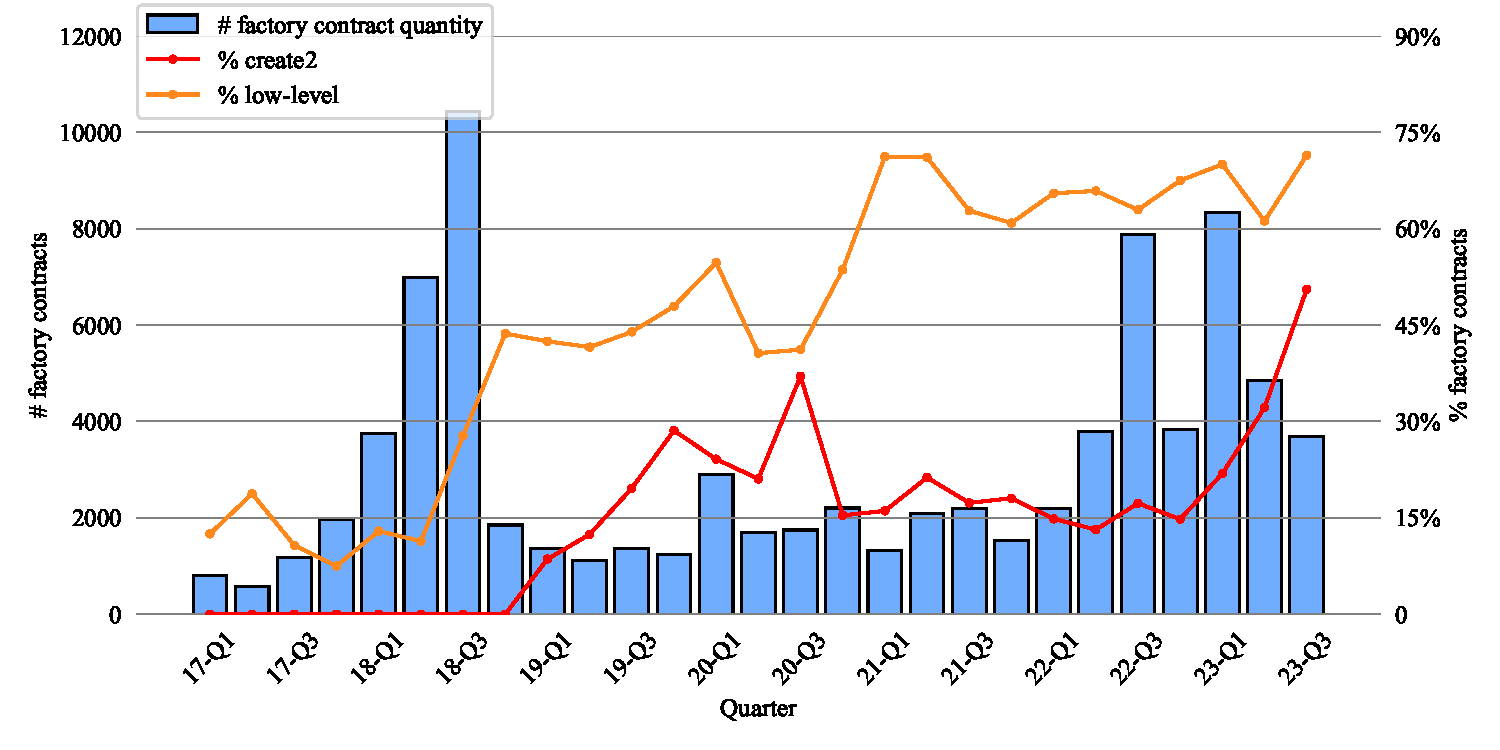
\includegraphics[width=0.85\linewidth]{figures/factory_contracts.pdf}
		\caption{Number of factory contracts deployed on the Ethereum mainnet.}
		\label{fig:factorydeploy}
	\end{figure}

	\begin{figure}[h]
		\centering
		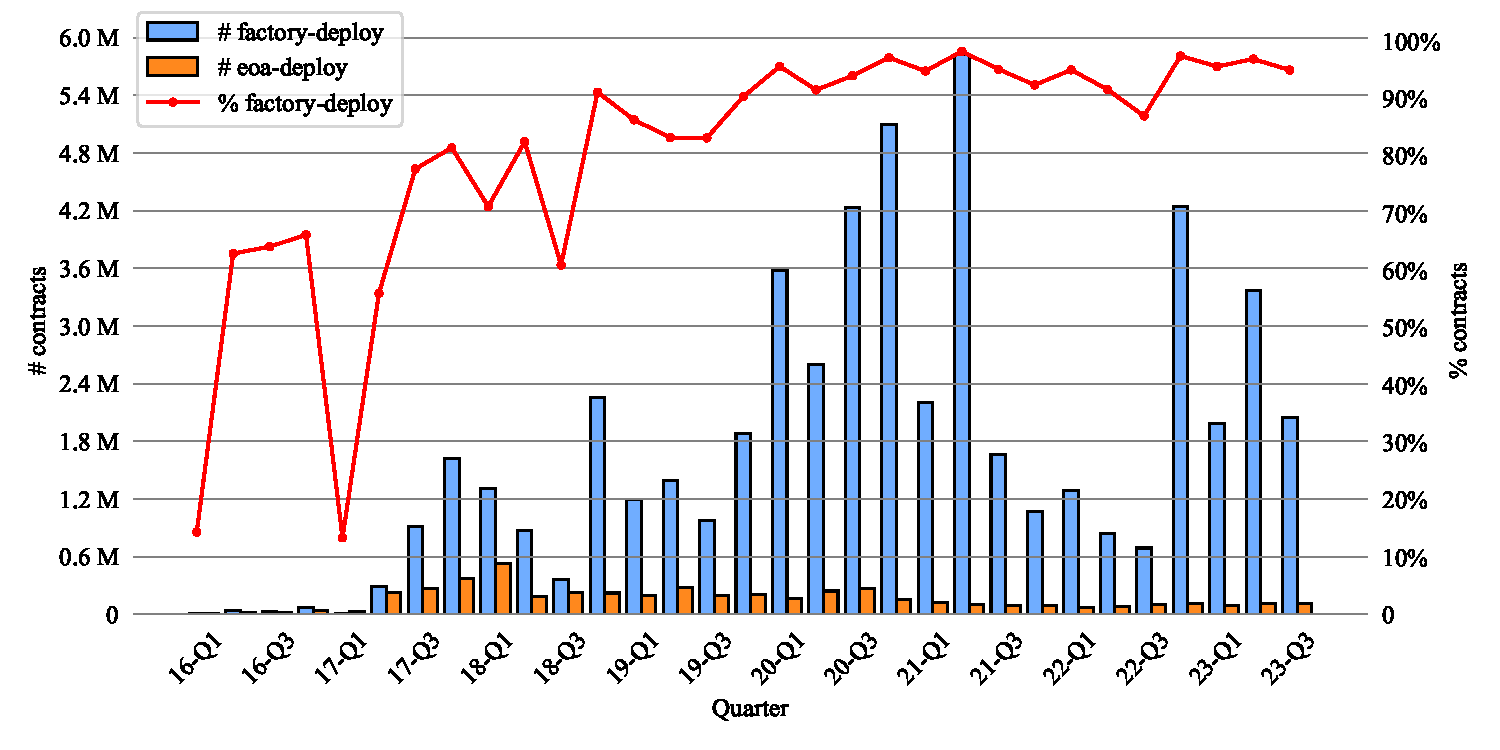
\includegraphics[width=0.85\linewidth]{figures/deployedcontracts.pdf}
		\caption{Comparison of trends for factory-deployed contracts and EOA-deployed contracts on Ethereum mainnet.}
		\label{fig:deployedcontracts}
	\end{figure}

	\section{Empirical Findings}\label{sec:findings}
	In this section, we present our empirical findings to address the three research questions.

	\subsection{RQ1: Prevalence}
	\textit{Factory quantity.}
	Figure ~\ref{fig:factorydeploy} shows the deployment count of factories on the Ethereum mainnet. The peak is in mid-2018, with nearly 5,000 contracts in July, driven by lending, stablecoin issuance, and decentralized trading. Despite a subsequent decline, annual deployments increased overall. The Constantinople fork in January 2019 introduces the \textit{create2} opcode, which offers more flexibility and changed deployment methods. In our dataset, post-January 2019, 49.8\% of contracts are deployed using \textit{create2}. It is worth noting that until the release of Solidity 0.7.0 in July 2020, access to the \textit{create2} opcode is restricted to inline assembly. Between July 2021 and October 2023, an average of 66.1\% of factories utilize inline assembly. The increase in the prevalence of such factories can be attributed to this constraint.


	\textit{Factory-deployed contract tendency.} Figure ~\ref{fig:deployedcontracts} shows  the Ethereum mainnet contract deployment from 2016 to 2024. EOA deployments peak in early 2018, then stabilized around 50,000 per month.  In contrast, Factory deployments increased significantly from 2017 to 2022, peaking at 2.5 million in June 2021. Early Ethereum development sees 85.2\% of contracts deployed by EOAs before mid-2016, but from January 2020 to October 2023, 92.7\% are deployed by factories. A downturn from 2021 to 2022 reflects the cryptocurrency bear market, cooling DeFi and NFT trends. Complete data is available on our Dune dashboard \cite{dunedashboard}.

	\begin{figure}[h]
		\centering
		\includegraphics[width=0.6\linewidth]{figures/clustered_semantic_space.pdf}
		\caption{Scatter plot of four clusters after dimensionality reduction.}
		% \label{fig:deployedcontracts}
	\end{figure}

	\textit{Factory contract application domains.} By conducting a cluster analysis on the collected FSCs, we identify four relatively clear clusters and categorize the remainder as miscellaneous. Upon manually reviewing the clustering outcomes, we discern the principal applications of FSCs and have encapsulated them in Table \ref{tab:clustering-results}, predominantly spanning four categories: \textit{Finance and Investment}, \textit{NFT-Related}, \textit{Decentralized and Infrastructure}, and \textit{Proxy and Forwarding}. Then we describe their main uses in detail and provide examples.


	\begin{itemize}[leftmargin=0.4cm,topsep=0.1cm]
		\item The \textit{finance and investment} category primarily involves smart contract functions related to financial transactions, asset management, investment strategies, crowdfunding, and fundraising. Classic protocol abbreviations and financial transaction-related vocabulary frequently appear in the contract names and function bodies of this category.
		\item The \textit{NFT-related} category mainly pertains to the creation, trading, showcasing, and management of Non-Fungible Tokens (NFTs). This domain encapsulates the burgeoning field of digital art and collectibles, gaming items, and other unique digital assets that are verified on the blockchain, ensuring authenticity and ownership.
		\item The \textit{decentralized and infrastructure} category includes building and maintaining the infrastructure for decentralized networks and applications, such as exchanges, liquidity pools, protocols, and contract management.  The backbone of the decentralized ecosystem enables the creation of distributed applications  that operate without a central authority, providing services like decentralized trading platforms and other protocol layers that ensure the smooth functioning and interoperability of various blockchain-based services.
		\item The \textit{proxy and forwarding} category relates to functionalities associated with proxy services, message forwarding, contract upgrades, and cross-contract communication. This category encapsulates smart contract patterns that allow for the upgradeability of contracts without changing their address, which is crucial for long-term maintenance and improvement.
	\end{itemize}

	\begin{table}[t]
  \centering
  \setlength{\extrarowheight}{1pt}
  \caption{Clustering Results for  Application Domains}
  \label{tab:clustering-results}
  \scriptsize % 改为 \scriptsize
  \begin{tabular}{|m{0.1\textwidth}|m{0.18\textwidth}|m{0.145\textwidth}|m{0.395\textwidth}|>{\centering\arraybackslash}m{0.05\textwidth}|}
    \hline
    \textbf{Category}\centering &  \textbf{Keywords} \centering & \textbf{EIP Protocols}\centering & \textbf{Representative Contract}\centering & \textbf{Number}  \\ 
    \hline
    Finance and Investment\centering &
    ico, dividend, wallet, account, trade, finance, fund, vesting &
    ERC-20, ERC-1155, ERC-4626, ERC-4980 &
    \texttt{CryptoFundManager,  DividendDistributor}&
    3424 \\
    \hline
    NFT Related\centering &
    art, mint, creator, trade, game, nft, digital, collectible & ERC-721, ERC-2981 &
    \texttt{CryptoArtCollection, NFTMintingPlatform}&
    1171 \\
    
    \hline
    Decentralized Infrastructure\centering &
    authority, defi, dapp, controller, node,  indelible, dao, uniswap & ERC-223 &
    \texttt{DecentralizedExchange, DeFiProtocolManager}&
    2225\\
    \hline
    Proxy Pattern\centering &
    upgradeable, relay, broker, router, middleman, forward, provider, delegate,  mediator, hypervisor &
    ERC-1967, ERC-1167 &
    \texttt{UpgradeableContract, WyvernProxyRegistry} &
    613 \\
    
    \hline
    Sum (\%) \centering &
    ---\centering &
    ---\centering &
    ---\centering &
    7433 (56.7\%) \\
    \hline
  
    % Blank and Unclassified\centering & Categories with missing function names or bodies and those that cannot be classified into a specific domain & test123, abc &  & 46.8\% \\
    % \hline
  \end{tabular}
\end{table}

	In Table~\ref{tab:clustering-results}, the "Keywords" column lists the tokens obtained from tokenizing the contract functions within the clustering results, where the frequency of each token exceeds fifty occurrences. The "Proxy" column represents manually categorized EIP protocols, which often appear explicitly in contract names. For instance, the \textit{ERC20} protocol represents a specific type of cryptocurrency token on the Ethereum blockchain, defining a set of rules that tokens must follow to facilitate transactions. Therefore, we classify it under the Finance and Investment category. The "Function Name Examples" column provides examples of contract function names for each category, allowing for a direct and intuitive understanding of the strong relevance to the respective domains.The aforementioned four categories account for 53.2\% of the total count. The remaining constarts include those with blank contract names or function bodies (14.9\%) and contracts with no clear semantics or undefined application domains (38.3\%).


	\begin{answerbox}
		\textbf{Answer to RQ1:} The Ethereum mainnet has deployed over 88,000 factory contracts, with 49.8\% utilizing the create2 opcode since the Constantinople upgrade. Furthermore, since 2020, over 92.7\% of contracts have been deployed by factories. These factories are primarily used in four scenarios.
	\end{answerbox}


	\subsection{RQ2: Functionalities and Patterns}\label{sec:4.3}
	We ultimately identify 20 low-level functionalities covering all smart contract components. A comprehensive list is presented on our repository \cite{fscdata}. Table~\ref{tab:patterns} details 6 factory-based patterns, their motivations, utilized functionalities, and quantities observed in our dataset.

% \begin{table}[h]
\caption{Manual Review Guidelines for Factory Decomposition}
\label{tab:imp}
\scriptsize
\resizebox{\textwidth}{!}{%
\begin{tabular}{|
>{\columncolor[HTML]{FFFFFF}}c |
>{\columncolor[HTML]{FFFFFF}}c |
>{\columncolor[HTML]{FFFFFF}}c |
>{\columncolor[HTML]{FFFFFF}}c |
>{\columncolor[HTML]{FFFFFF}}c |}
\hline
\textbf{Functionalities} &
  ID &
  Sub-Functionalities &
  Real World Implementations &
  Related Contract Component \\ \hline
\cellcolor[HTML]{FFFFFF} &
  \cellcolor[HTML]{FFFFFF} &
  \cellcolor[HTML]{FFFFFF} &
  low-level:create opcode &
  \cellcolor[HTML]{FFFFFF} \\ \cline{4-4}
\cellcolor[HTML]{FFFFFF} &
  \cellcolor[HTML]{FFFFFF} &
  \cellcolor[HTML]{FFFFFF} &
  low-level:create2 opcode &
  \cellcolor[HTML]{FFFFFF} \\ \cline{4-4}
\cellcolor[HTML]{FFFFFF} &
  \multirow{-3}{*}{\cellcolor[HTML]{FFFFFF}F1} &
  \multirow{-3}{*}{\cellcolor[HTML]{FFFFFF}Methods of deploying contracts} &
  high-level:new Contract &
  \multirow{-3}{*}{\cellcolor[HTML]{FFFFFF}Functions} \\ \cline{2-5} 
\cellcolor[HTML]{FFFFFF} &
  \cellcolor[HTML]{FFFFFF} &
  \cellcolor[HTML]{FFFFFF} &
  delay time deployment &
  Modifiers, Functions \\ \cline{4-5} 
\cellcolor[HTML]{FFFFFF} &
  \multirow{-2}{*}{\cellcolor[HTML]{FFFFFF}F2} &
  \multirow{-2}{*}{\cellcolor[HTML]{FFFFFF}Deployment timing} &
  Immediate deployment &
  Functions \\ \cline{2-5} 
\cellcolor[HTML]{FFFFFF} &
  \cellcolor[HTML]{FFFFFF} &
  \cellcolor[HTML]{FFFFFF} &
  template-based factory passes parameter in created contract constructor &
  \cellcolor[HTML]{FFFFFF} \\ \cline{4-4}
\cellcolor[HTML]{FFFFFF} &
  \cellcolor[HTML]{FFFFFF} &
  \cellcolor[HTML]{FFFFFF} &
  template-based factory call Initialization function after deployment &
  \cellcolor[HTML]{FFFFFF} \\ \cline{4-4}
\cellcolor[HTML]{FFFFFF} &
  \cellcolor[HTML]{FFFFFF} &
  \cellcolor[HTML]{FFFFFF} &
  bytecode-based factory accepts contract bytecode as parameter &
  \cellcolor[HTML]{FFFFFF} \\ \cline{4-4}
\multirow{-9}{*}{\cellcolor[HTML]{FFFFFF}\begin{tabular}[c]{@{}c@{}}Contract \\ Deployment\end{tabular}} &
  \multirow{-4}{*}{\cellcolor[HTML]{FFFFFF}F3} &
  \multirow{-4}{*}{\cellcolor[HTML]{FFFFFF}Created contract customization} &
  clone-based factory based on target address contract bytecode &
  \multirow{-4}{*}{\cellcolor[HTML]{FFFFFF}Functions} \\ \hline
\cellcolor[HTML]{FFFFFF} &
  \cellcolor[HTML]{FFFFFF} &
  \cellcolor[HTML]{FFFFFF} &
  check extcode &
  \cellcolor[HTML]{FFFFFF} \\ \cline{4-4}
\cellcolor[HTML]{FFFFFF} &
  \cellcolor[HTML]{FFFFFF} &
  \cellcolor[HTML]{FFFFFF} &
  check address equal 0 &
  \cellcolor[HTML]{FFFFFF} \\ \cline{4-4}
\cellcolor[HTML]{FFFFFF} &
  \multirow{-3}{*}{\cellcolor[HTML]{FFFFFF}F4} &
  \multirow{-3}{*}{\cellcolor[HTML]{FFFFFF}\begin{tabular}[c]{@{}c@{}}Check the validity of the \\ created contract address\end{tabular}} &
  check address equal to target address &
  \multirow{-3}{*}{\cellcolor[HTML]{FFFFFF}Events, Functions} \\ \cline{2-5} 
\cellcolor[HTML]{FFFFFF} &
  \cellcolor[HTML]{FFFFFF} &
  \cellcolor[HTML]{FFFFFF} &
  owner signature verify &
  \cellcolor[HTML]{FFFFFF} \\ \cline{4-4}
\multirow{-5}{*}{\cellcolor[HTML]{FFFFFF}\begin{tabular}[c]{@{}c@{}}Validity \\ Check\end{tabular}} &
  \multirow{-2}{*}{\cellcolor[HTML]{FFFFFF}F5} &
  \multirow{-2}{*}{\cellcolor[HTML]{FFFFFF}\begin{tabular}[c]{@{}c@{}}Check the validity of the \\ created contract configuration\end{tabular}} &
  owner address verify &
  \multirow{-2}{*}{\cellcolor[HTML]{FFFFFF}Modifiers, Functions} \\ \hline
\cellcolor[HTML]{FFFFFF} &
  \cellcolor[HTML]{FFFFFF} &
  \cellcolor[HTML]{FFFFFF} &
  set up roles in factory constructor &
  \cellcolor[HTML]{FFFFFF} \\ \cline{4-4}
\cellcolor[HTML]{FFFFFF} &
  \multirow{-2}{*}{\cellcolor[HTML]{FFFFFF}F6} &
  \multirow{-2}{*}{\cellcolor[HTML]{FFFFFF}Role empowerment} &
  grand role to specified address &
  \multirow{-2}{*}{\cellcolor[HTML]{FFFFFF}State Variables, Functions} \\ \cline{2-5} 
\multirow{-3}{*}{\cellcolor[HTML]{FFFFFF}\begin{tabular}[c]{@{}c@{}}Access \\ Control\end{tabular}} &
  F7 &
  Deployer permission detection &
  require sender has role to deploy contract &
  Modifiers \\ \hline
\cellcolor[HTML]{FFFFFF} &
  \cellcolor[HTML]{FFFFFF} &
  \cellcolor[HTML]{FFFFFF} &
  use map/array to track and store which addresses have been deployed &
  \cellcolor[HTML]{FFFFFF} \\ \cline{4-4}
\cellcolor[HTML]{FFFFFF} &
  \multirow{-2}{*}{\cellcolor[HTML]{FFFFFF}F8} &
  \multirow{-2}{*}{\cellcolor[HTML]{FFFFFF}\begin{tabular}[c]{@{}c@{}}Created contract managed \\ internal factory\end{tabular}} &
  Mapping of the deployer address to an array of all deployed contracts &
  \multirow{-2}{*}{\cellcolor[HTML]{FFFFFF}State Variables} \\ \cline{2-5} 
\multirow{-3}{*}{\cellcolor[HTML]{FFFFFF}\begin{tabular}[c]{@{}c@{}}Tracking \&\\ Maintenance\end{tabular}} &
  F9 &
  \begin{tabular}[c]{@{}c@{}}Created contract managed \\ external factory\end{tabular} &
  emit deployed contract address to the upper layer application &
  Events \\ \hline
\end{tabular}%
}
\end{table}

	\textit{Template Configuration Pattern.} This is the most fundamental pattern in FSCs, implemented by 52.9\% (1967/3718) of factory contracts. It deploys multiple instances of contracts with identical runtime bytecode. The pattern dictates that the factory should deploy new contracts based on a predefined template and configure new instances via constructor parameters or initialization methods post-deployment. This pattern is widely utilized in various dApps, such as ERC-20 token contracts and ERC-721 NFT contracts.
	Two main implementation methods exist: using the \textit{new} keyword (e.g., \textit{new Token(strategy, expiration, decimal)}) or using \textit{create} or \textit{create2} in inline assembly. For instance, UniswapV2Factory \cite{uniswapv2factory} shown in Figure~\ref{lst:uniswap} uses \textit{create2(0,add(),mload(),salt)} to create new pair contracts, followed by initialization with \textit{IUniswapV2Pair(p).initialize(t0,t1)}.

	\begin{figure}[h]
		\begin{minipage}{\linewidth}
			\begin{lstlisting}
function createPair(address tokenA, address tokenB) external returns (address pair) {
  bytes memory bytecode = type(UniswapV2Pair).creationCode;
  bytes32 salt = keccak256(abi.encodePacked(token0, token1));
  assembly {
    pair := create2(0, add(bytecode, 32), mload(bytecode), salt)
  }
  IUniswapV2Pair(pair).initialize(token0, token1);
  getPair[token0][token1] = pair;
  getPair[token1][token0] = pair;
  allPairs.push(pair);
  emit PairCreated(token0, token1, pair, allPairs.length);
}
			\end{lstlisting}
		\end{minipage}
		\caption{Code snippet of the UniswapV2Factory contract, which uses the bytecode of UniswapV2Pair to deploy new trading pair contracts.}
		\label{list:uniswap}
	\end{figure}


	\begin{figure}[h]
		\begin{minipage}{\linewidth}
			\begin{lstlisting}
function cloneDeterministic(address implementation,bytes32 salt,uint256 value) internal{
  assembly ("memory-safe") {
    //Cleans the upper 96 bits of the `implementation` word, then packs the first 3 bytes of the `implementation` address with the bytecode before the address.
    mstore(0x00, or(shr(0xe8, shl(0x60, implementation)), 0x3d602d80600a3d3981f3363d3d373d3d3d363d73000000))
    //Packs the remaining 17 bytes of `implementation` with the bytecode
    mstore(0x20, or(shl(0x78, implementation), 0x5af43d82803e903d91602b57fd5bf3))
    instance := create2(value, 0x09, 0x37, salt)
  }
  if (instance == address(0)) {
    revert Errors.FailedDeployment();
  }
}
			\end{lstlisting}
		\end{minipage}
		\caption{Code snippet of the OpenZeppelin Clones contract, this function creates a minimal proxy of the implementation contract.}
		\label{list:clone}
	\end{figure}




	\textit{Proxy Delegation Pattern.} While the Template Configuration Pattern is a simple way to deploy multiple instances, storing the bytecode of each contract repeatedly can significantly increase gas costs. This pattern mitigates gas costs associated with storing repeated bytecode by deploying one master contract instance. All other instances act as proxies, delegating calls to the master while maintaining independent states.

	We analyze the implementation methods and quantities of this pattern in our dataset. Among 751 detected patterns, 73.23\% (550 / 751) of factories use @openzeppelin/contracts/proxy/Clones.sol to deploy minimal proxy contracts. Figure~\ref{list:clone} shows the code snippet of the Clones contract, which follows EIP-1167 (Minimal Proxy Contract) \cite{eip-1167}. This factory contract creates a minimal proxy contract of a specified implementation contract, which uses minimal bytecode to delegate calls to a fixed address, optimizing gas costs. However, unverified master contract addresses could pose security risks, discussed in Section~\ref{sec:security-senderconst}.

	\begin{table}[t]
	\centering
	\setlength{\extrarowheight}{1pt}
	\caption{Identified Factory-based Patterns}
	\label{tab:patterns} \scriptsize
	\begin{tabular}{|m{0.114\textwidth}|m{0.36\textwidth}|m{0.36\textwidth}|}
		\hline
		\textbf{Pattern Name}\centering & \textbf{Motivation}\centering                                                                           & \textbf{Used Functionalities}                                                                                                                                 \\
		\hline
		Template Configuration Pattern  & Facilitate efficient deployment and configuration of identical contracts                                & Use new or \textit{create} / \textit{create2} to deploy contracts. Then call init\_function or pass parameters to the constructor for contract initialization \\
		\hline
		Proxy Delegation Pattern        & Optimize gas costs by deploying minimal proxy contracts for identical contracts                         & Use Clones library to deploy minimized proxy contracts. Validate the untrusted master contract                                                                \\
		\hline
		Centralized Registry Pattern    & Improve management efficiency and traceability of deployed contracts through a centralized approach     & Use \textit{map} / \textit{array} to store and keep track of all deployed contracts. Check which contracts have been previously deployed                      \\
		\hline
		Keyless Singleton Pattern       & Deploy contracts with the same init code to the same address in multiple blockchains                    & Use Nick's method to deploy keyless factories. Utilize \textit{create2} for deterministic contract address independent of deployer's nonce                    \\
		\hline
		Salted Address Pattern          & Calculating the contract address requires only the deployer's address and salt, excluding initcode hash & Utilize \textit{create2} opcode for deterministic contract address independent of deployer account's nonce                                                    \\
		\hline
		Metamorphic Factory Pattern     & Support contract upgradeability and some malicious purposes                                             & Use \textit{selfdestruct} opcode to clear contract code and storage. Use a transient factory to deploy metamorphic contracts                                  \\
		\hline
	\end{tabular}
\end{table}


	\textit{Centralized Registry Pattern.} This pattern enhances the management and traceability of deployed contracts by using a central registry contract to store the addresses of deployed contract instances along with their associated information, such as version and owner details. It simplifies the operations of contract factories, making querying and verification more convenient. Additionally, it lays the groundwork for advanced functionalities like access control.
	WyvernProxyRegistry, the contract with the highest transaction volume among factories in our dataset, exemplifies this pattern. It is used to identity verification and access control on the trading platform Wyvern. It uses $mapping(address \Rightarrow OwnableDelegateProxy)$ public proxies to centrally manage user-verified proxies. Users can create a new AuthenticatedProxy contract via \textit{registerProxy()} and adding it to the registry.


	\textit{Keyless Singleton Pattern.} Some dapps require deploying contract instances to the deterministic address across multiple blockchains, such as contracts adhering to the EIP-1820 (Universal Registry Contract) \cite{eip-1820}. This pattern, proposed in ERC-2470 (Singleton Factory) \cite{eip-2470}, and its core involves adopting Nick's method \cite{nickmethod} to deploy factory contracts. This method ensures a deterministic address deployment across blockchains using Nick's method \cite{nickmethod}.

	Therefore, developers can deploy contract instances with the same initialization code to the same address on different chains using such create2 factories. This is because when deploying a contract with create2, the contract's address is determined by the factory address, salt, and initcode. With the factory address constant across chains, using the same salt ensures the same deployed contract address. In total, we find 166 factory contracts implement this pattern. These contracts have the same address on the Ethereum mainnet, as well as on the Sepolia \cite{sepolia} and Goerli \cite{goerli} testnets.

	\textit{Salted Address Pattern.} Some deployers prefer the deployed contract's address not to depend on the hash of the initialization code. For this purpose, the EIP-3171 \cite{eip-3171} introduced the pattern, called Create3 Factory. This pattern ensures that the address of the deployed contract is only determined by the deployer's address and the salt. More importantly, compared to the limitations of the Keyless Singleton Pattern, this pattern allows deployers to conveniently deploy contract instances with different initialization codes to the same address across multiple blockchains. Additionally, contracts deployed through this pattern retain predictability.

	\textit{Metamorphic Factory Pattern.} Immutable code is considered to be the cornerstone of a stable blockchain ecosystem. However, the emergence of the Metamorphic Factory Pattern disrupts this rule. It uses a metamorphic factory to smoothly upgrade factory-deployed contracts without changing the deployed contract address, offering viable support for maintenance, fixes, and upgrades across multiple chains. Unlike the contract upgrade standards specified by protocols like ERC-1822 (Universal Upgradeable Proxy Standard) \cite{eip-1822}, contracts deployed by metamorphic factory, once upgraded, will delete all existing storage and replace the existing code with the new implementation code. Figure~\ref{lst:metamorphic} presents a concise implementation of metamorphic pattern. The \textit{deployMetamorphic()} function utilizes the \textit{create2} opcode to deploy TransientFactory. Within the temporary factory's constructor, first deploy the metamorphic contract using the create opcode, followed by the execution of a self-destruct operation, resetting the transient factory's nonce. When the metamorphic contract needs to be replaced, first execute the \textit{selfdestruct} operation on it. Then call the \textit{deployMetamorphic()} again, and make sure we pass in the same salt as before. The TransientFactory will redeploy the new metamorphic contract code to the same address to achieve the seamless contract replacement.

	\begin{figure}[t]
		\begin{minipage}{\linewidth}
			\begin{lstlisting}
contract MetamorphicContractFactory {
  bytes private transientFactoryCode;
  mapping(address => bytes) private initCodes;
  function deployMetamorphic(bytes32 salt,bytes metamorphicInitCode) external payable {
    address tempFactory;
    assembly {
      let d:=add(0x20, metamorphicInitCode)
      let s:=mload(metamorphicInitCode)
      tempFactory:=create2(callvalue,d,s,salt)
    }
    initCodes[tempFactory]=metamorphicInitCode;
  }
}
contract tempFactory {
  constructor() public payable {
    bytes initCode = IFactory(msg.sender).getInitCode();
    assembly {
      let d := add(0x20,initCode)
      let s := mload(initCode)
      metamorphicAddr := create(callvalue,d,s)
    }
    selfdestruct(metamorphicAddr);
  }
}
			\end{lstlisting}
		\end{minipage}
		\caption{An implementation of metamorphic pattern.}
		\label{lst:metamorphic}
	\end{figure}



	However, this pattern has become a weapon for certain malicious activities, presenting new challenges to smart contract security. In Section~\ref{sec:security-mutablecode}, we will discuss its attack vectors and corresponding countermeasures in detail.
	\begin{answerbox}
		\textbf{Answer to RQ2:} Six factory-based patterns are identified, covering over 3,718 factories. Notably the Template Configuration Pattern and Proxy Delegation Pattern account for 52.9\% and 20.2\% respectively, highlighting the significance of factories for multiple instances deployment.
	\end{answerbox}

	\subsection{RQ3: Security Risks and Case Studies}\label{sec:rq4securityrisks}

	\newcolumntype{R}{>{\raggedleft\arraybackslash}X} % Define the "R" column type
\begin{table}[htbp]
  \centering
  \footnotesize
  \caption{Detected Security Issues Related to Factory Contracts}
  \label{tab:security}
  \begin{tabularx}{0.6\linewidth}{@{}lR@{}}
    \toprule
    \textbf{Issue Name}                     & \textbf{Number} \\
    \midrule
    (1) Mutable Code                   & 91     \\
    (2) Unexpected Ownership Transfer & 267    \\
    (3) Unhandled Low-Level Contract Creation & 600    \\
    (4) Unverified Master Contract       & 222    \\
    \bottomrule
  \end{tabularx}
\end{table}


	We ultimately find 1,180 real-world smart contracts with four type of security issues using developed detectors. Table~\ref{tab:security} illustrates the security issues quantities across networks. The first two pertain to factory-deployed contract issues, and the latter two to factory contract issues. Next, we present in-depth case studies, outlining impacts and solutions.

	\subsubsection{Mutable Code}\label{sec:security-mutablecode}
	The on-chain smart contract code is conventionally considered immutable. Yet, the introduction of the \textit{create2} opcode has given rise to specific factory-based patterns that facilitate contract mutability, which implies that the code can change in-place post-deployment. Previous research employs the term Metamorphic Contracts \cite{DBLP:conf/fc/FrowisB22} to categorize contracts featuring this particular characteristic.

	Although the emergence of metamorphic contracts offers an implementation approach for upgradeable contracts, it also creates new opportunities for attackers to engage in malicious activities. While metamorphic contracts themselves may not contain inherent vulnerabilities, significant security challenges arise from the interaction of other contracts and externally owned accounts with them. For example, users who previously interacted with a seemingly benign token-staking contract could suddenly find themselves interacting with a malicious contract that includes token-stealing functionalities.

	In the following, we will first conduct a case study of the Tornado Cash governance attack \cite{tornado-cash-attack}, in which the attacker leveraged the metamorphic pattern to carry out the attack, and then provide a simplified implementation of the metamorphic pattern.

	\begin{figure}[h]
		\centering
		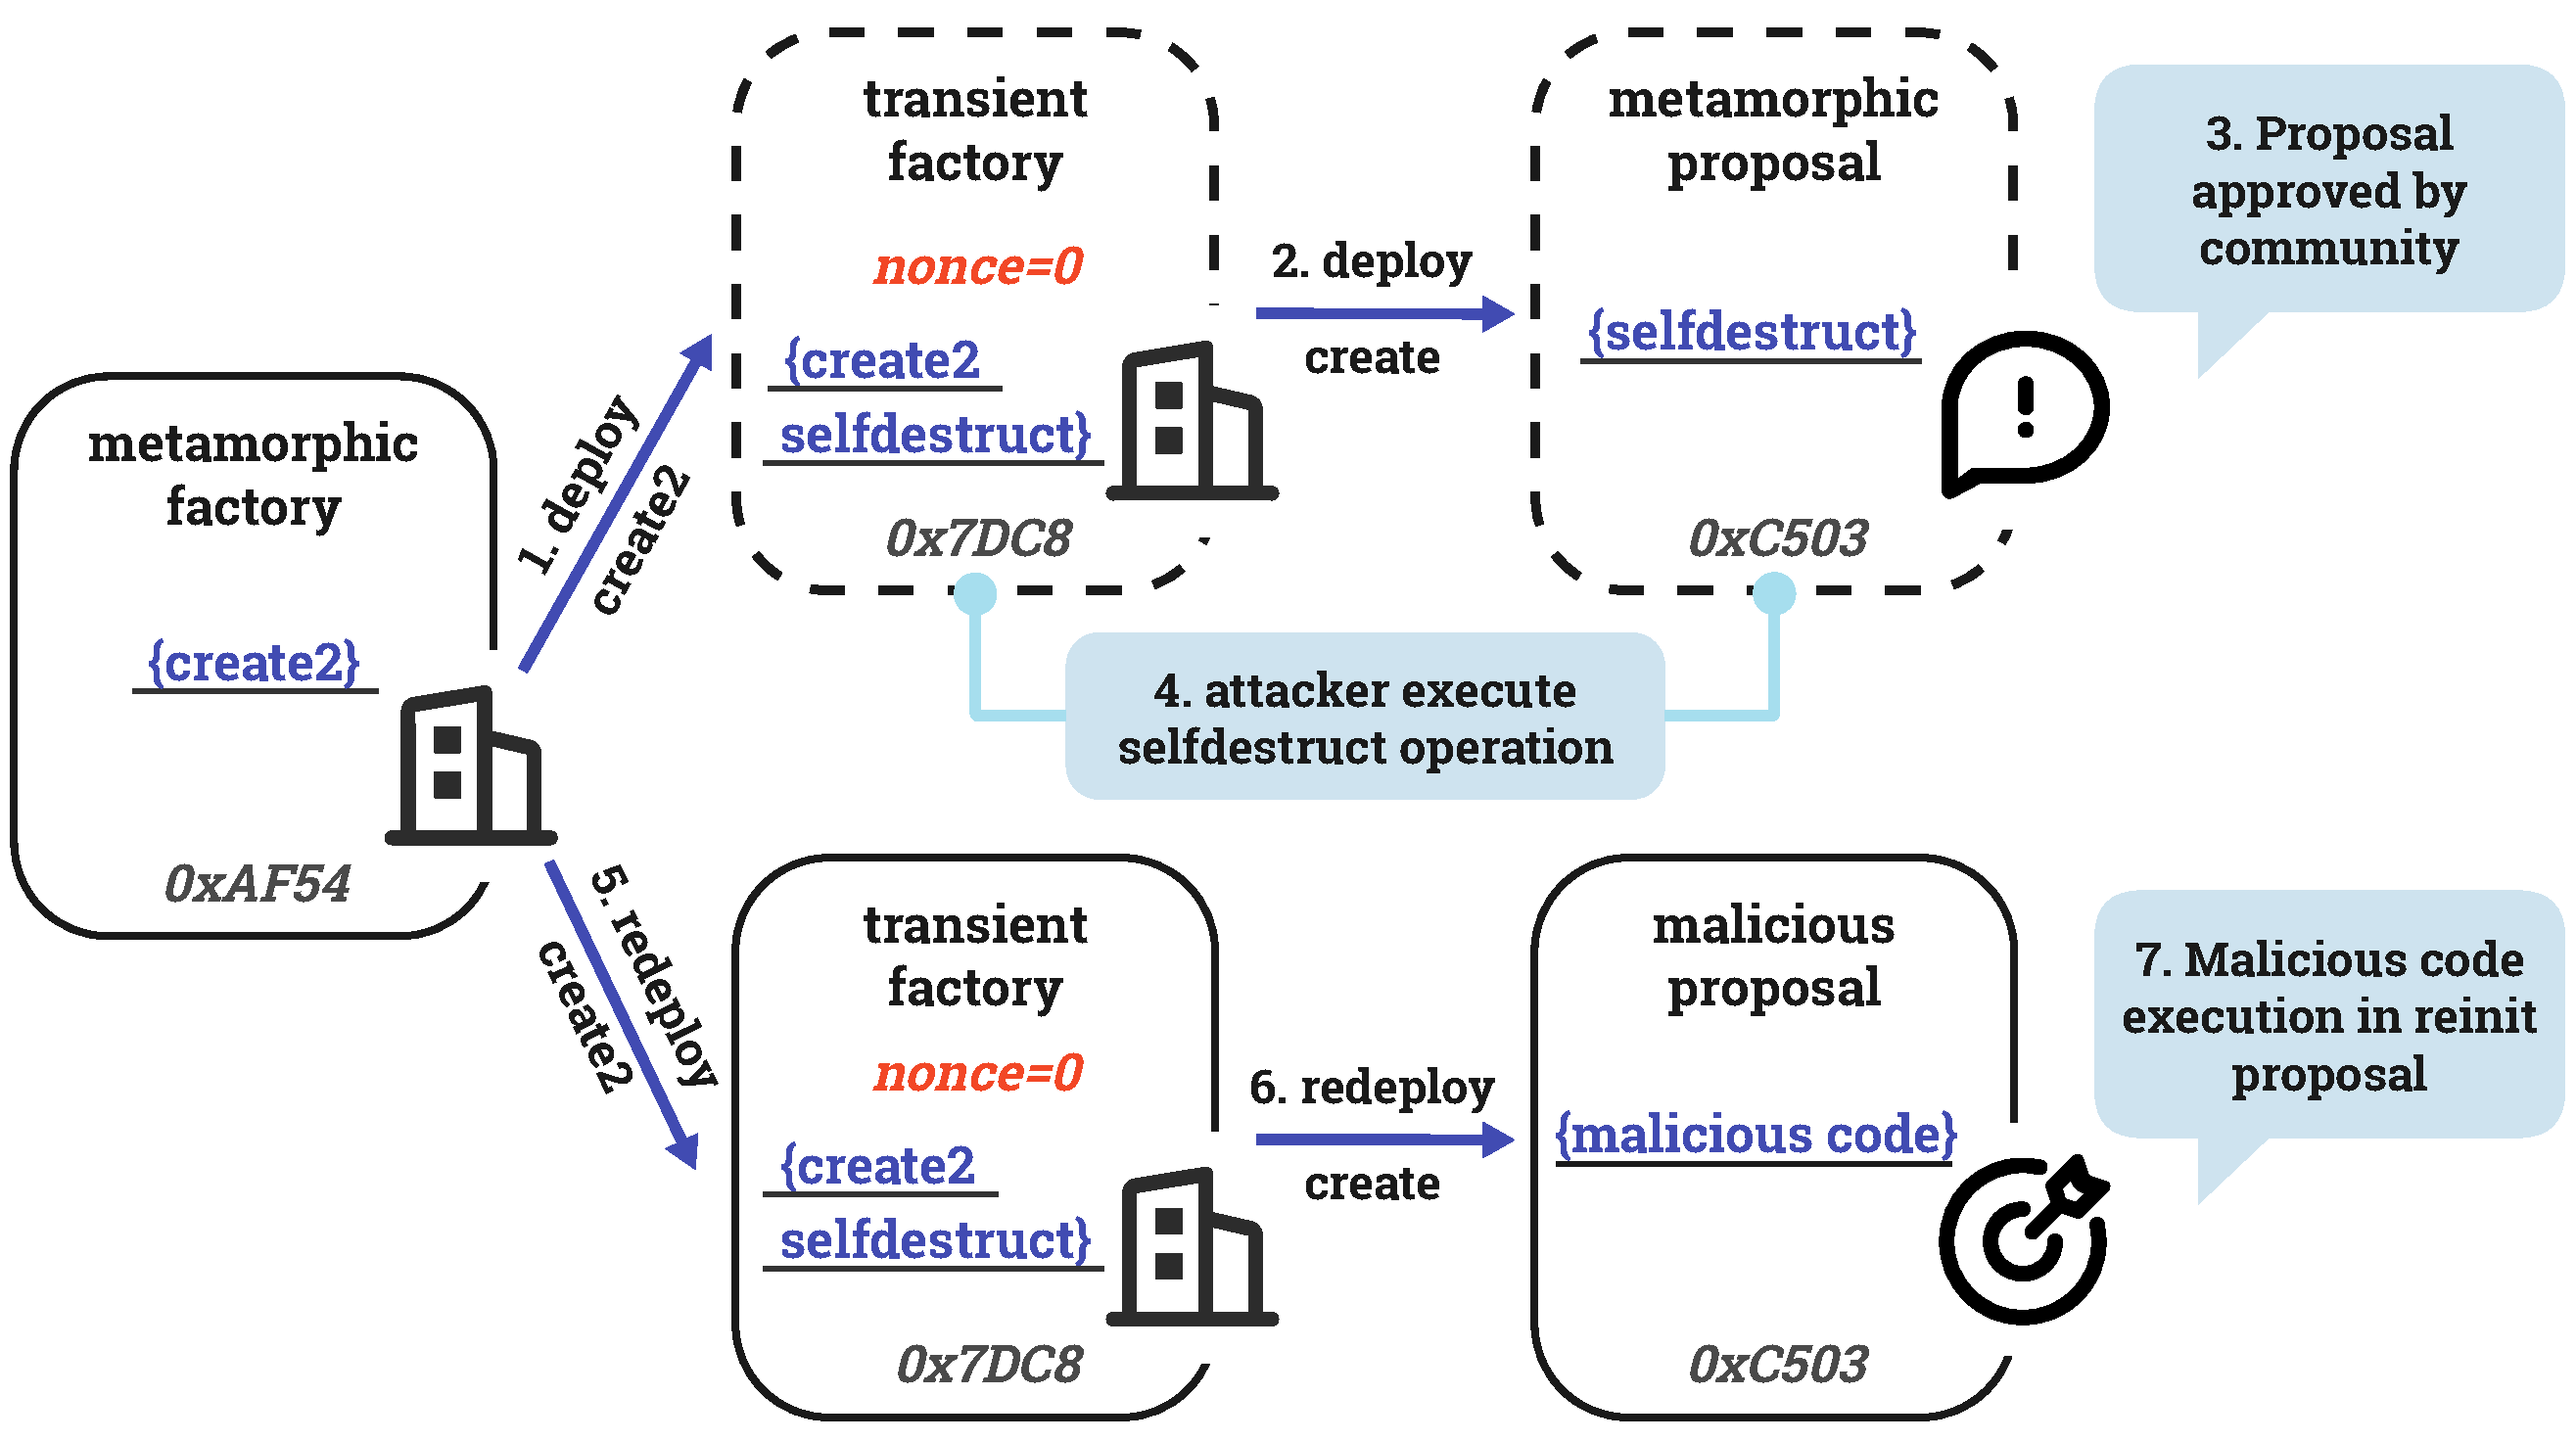
\includegraphics[width=0.85\linewidth]{figures/attack.pdf}
		\caption{The process of Tornado Cash DAO attack.}
		\label{fig:tornado_attack}
	\end{figure}


	Figure~\ref{fig:tornado_attack} illustrates the steps of the attack: \ding{172} The attacker first utilizes the \textit{create2} opcode of the disguised factory to deploy a transient factory, which includes \textit{selfdestruct} and \textit{create} opcodes. \ding{173} Next, the transient factory uses \textit{create} opcode to deploy a seemingly harmless proposal contract, which also contains \textit{selfdestruct}. \ding{174} The proposal is approved and becomes executable. \ding{175} The attacker executes \textit{selfdestruct} on both the transient factory and the proposal. \ding{176} The attacker then redeploys the transient factory, maintaining the same salt and bytecode. This results in the transient factory having the same address as before, with the nonce value reset. \ding{177} Subsequently, the attacker employs the \textit{create} opcode of the transient factory to deploy a modified malicious proposal at the address of the previous proposal. \ding{178} Finally, the attacker executes the malicious code within the proposal, leading to fund theft. This attack highlights the complexity and subtlety of security issues associated with FSCs, which consequently inspires our research to focus on FSC patterns and security risks.

	\begin{algorithm}
		\caption{Detect Metamorphic Contract}\label{alg:detect_metamorphic_contract}
		\begin{algorithmic}[1]
			\Statex \textbf{Input:} $target$ $contract$ $address$
			\Statex \textbf{Output:} Boolean indicating whether the contract is metamorphic
			\Procedure{detectMetamorphicContract}{$address$, $network$, $db\_client$}
				\State $runtime\_code \gets \text{fetch\_contract\_bytecode}(network, address)$
				\If{(not $runtime\_code$) or (not \text{is\_contract\_account}(runtime\_code))}
					\State \Return False
				\EndIf
				\State $contain\_selfdestruct \gets \text{contain\_opcode}(runtime\_code, \text{SELFDESTRUCT})$
				\State $contain\_delegatecall \gets \text{contain\_opcode}(runtime\_code, \text{DELEGATECALL})$
				\State $contain\_callcode \gets \text{contain\_opcode}(runtime\_code, \text{CALLCODE})$
				\If{not ($contain\_selfdestruct$ or $contain\_delegatecall$ or $contain\_callcode$)}
					\State \Return False
				\EndIf

				\While{True} \Comment{Construct Contract Deployment Chain}
				\State $creation \gets \text{find\_factory\_addr\_and\_create\_type}(network, cur\_node.address, db\_client)$
				% \If{not $creation$}
				% \EndIf
				\State $factory\_addr, create\_type \gets creation$
				\State $factory\_bytecode \gets \text{fetch\_contract\_bytecode}(network, factory\_addr)$
				\State $factory\_node \gets \text{ContractNode}(network, factory\_addr, factory\_bytecode)$
				\State $factory\_node.link\_succ(create\_type, cur\_node)$
				\State $cur\_node \gets factory\_node$
				\EndWhile
				\State $is\_metamorphic\_pattern \gets \text{detect\_metamorphic\_pattern}(target\_node)$
				\State \Return $is\_metamorphic\_pattern$
			\EndProcedure

			\Procedure{detectMetamorphicPattern}{$target\_node$}
				\If{$target\_node.created\_type == $ CREATE2}
					\State \Return False
				\EndIf
				\State $cur\_node \gets target\_node.prec$
				\While{$cur\_node$ is not None}
					\If{(SELFDESTRUCT or DELEGATECALL) not in cur\_node.bytecode}
						\State \Return False
					\EndIf
					\If{$cur\_node.created\_type == \text{'create2'}$}
						\State \Return True
					\EndIf
					\State $cur\_node \gets cur\_node.prec$
				\EndWhile
				\State \Return False
			\EndProcedure
		\end{algorithmic}
	\end{algorithm}



	\textit{Detection Method.}
	Algorithm~\ref{alg:detect_metamorphic_contract} outlines the process for detecting metamorphic contracts. Specifically, our detector first takes a target contract address as input. It begins by fetching the runtime bytecode of the target contract and verifies that it is indeed a contract account. If the target is not a contract account, the detector terminates the analysis and flags it as not metamorphic. Next, the detector analyzes the runtime bytecode for the presence of the \textit{selfdestruct}, \textit{delegatecall}, or \textit{callcode} opcodes. The presence of any of these opcodes indicates a potential for metamorphic behavior, and it is required for the contract to be metamorphic. If the initial checks pass, the detector proceeds to construct the contract deployment chain by iteratively tracing back to the factory contracts. The full deployment chain extends from the deployed contract, up to its top-level factory.


	Subsequently, the detector checks the chain to confirm the presence of the metamorphic pattern using the following algorithm. First, the detector analyzes whether the direct creator of the target contract was created via the \textit{create} opcode. If not, the target contract cannot be a metamorphic contract. Then, the detector examines the bytecode of the direct creator of the target contract to check if the \textit{selfdestruct} or \textit{delegatecall} opcodes are present. If these two opcodes are not present, the target contract cannot be a metamorphic contract. Subsequently, the detector further analyzes the entire contract deployment chain to determine if any contract was created by the \textit{create2} opcode. If any such contract is found, then the target contract is flagged as a metamorphic contract. If the end of the deployment chain is reached and no contracts created by the \textit{create2} opcode are found, then the detector returns false.


	\textit{Countermeasures.} In decentralized governance, it is crucial to be aware of the potential risks when interacting with external contracts (proposals). Before a contract's proposal is approved, it should be reviewed from the following perspectives: \ding{172} When interacting with a contract, ensure that the \textit{selfdestruct} opcode is absent and unreachable via \textit{delegatecall}. \ding{173} Validate the entire contract deployment chain and confirm the trusted origin of the interacting contract. \ding{174} Before calling an external contract, verify its \textit{extcodehash} to ensure its code hasn't changed. We conduct cross-contract analysis based on the contract deployment chain, revealing a total of 91 metamorphic factory-deployed contracts. We manually verify them to ensure no false positives. To enhance the security of Ethereum community governance, we make the dataset public in our repository \cite{fscdata}.

	\subsubsection{Unexpected Ownership Transfer}\label{sec:security-senderconst} When a contract is deployed, the initial ownership is usually established in the constructor, often with a statement like \textit{owner = msg.sender}. However, contracts deployed via a factory must not use the \textit{msg.sender} in constructor, instead use constructor parameters to specify the ownership. Failing to recognize this difference could inadvertently make the factory the only owner / controller of the deployed contract.


	Figure~\ref{lst:senderinconst} provides an example, including the NFTSample contract and a simplified version of Ownable from \textit{@openzeppelin/contracts/access/Ownable.sol}. In this context, NFTSample is deployed by a factory. During the deployment procedure, the constructor of Ownable is executed first, assigning \textit{owner} the factory address, not the EOA account. Consequently, the msg.sender in constructor of NFTSample and all its base contracts point to the address of the factory. This will lead to contamination of some state variables in the NFTSample. What's worse, since the \textit{withdrawMoney()} is protected by \textit{onlyOwner} modifier, the deployer subsequently loses any permission to call \textit{withdrawMoney()}. We totally find 408 contracts where ownership is unexpectedly transferred in the constructor in our dataset\cite{fscdata}. The reported vulnerability could be a false positive, as it may be intentionally designed by the deployer. As mentioned in Section~\ref{sec:4.3}, contracts following the EIP-1820 protocol may utilize a centralized registry to track all deployed contracts. Thus, deployed contracts could designate the factory contract as their owner in the constructor.

	\begin{figure}[t]
		\begin{minipage}{\linewidth}
			\begin{lstlisting}
abstract contract Ownable is Context {
  address private _owner;
  constructor() {
    transferOwnership(msg.sender);
  }
  function transferOwnership(address newOwner) public onlyOwner {
    require(newOwner != address(0));
    address oldOwner = _owner;
    _owner = newOwner;
  }
}
contract NFTSample is Ownable,ReentrancyGuard {
  constructor() {
    maxBatchSize = 8;
    collectionSize = 16384;
    _setDefaultRoyalty(_owner, 500);
    operatorFilteringEnabled = true;
  }
    function withdrawMoney() onlyOwner {...}
}
			\end{lstlisting}
		\end{minipage}
		\caption{Example of the transfer of contract ownership.}
		\label{lst:senderinconst}
	\end{figure}

	\textit{Detection Method.} To detect this security issue, our detector first determines whether the direct deployer of the target contract is a contract account or an externally owned account (EOA) by analyzing the contract deployment chain. If it is a contract account (a factory contract), the detector further analyzes the target contract's constructor. First, it checks if the constructor() includes an assignment operation to the owner state variable. If such an assignment exists, it performs a backward taint analysis to obtain the right-hand side value of that assignment statement. Finally, it checks if this right-hand side value includes the msg.sender variable. If it does, the target contract is flagged as having this security issue.

	\textit{Countermeasures.} To address this, some common patterns like Ownable should be modified to accommodate it. For example, we identify 2772 factory-deployed contracts inheriting from Ownable, with 324 of these execute \textit{transferOwnership(tx.origin)} at the end of  their constructors to retransferring ownership to EOA.


	\subsubsection{Unhandled Low-Level Contract Creation}
	When a factory fails to deploy a contract (due to address conflict, insufficient gas, or incorrect bytecode), using the \textit{new} keyword will cause the entire transaction to revert. If the factory uses \textit{create} / \textit{create2} opcode in inline assembly, these opcodes will return \textit{zero} address, and the transaction will continue executing silently. This type of issue can result in Ether being permanently locked in the factory if a developer uses factory to deploy contract and attaches Ether via msg.value. This underscores the necessity for factories deploying contracts via inline assembly to meticulously conduct checks on the deployed contract's address. Among the 1685 verified low-level factories with unique source code in our dataset, 798 contracts include address check. We categorize the checking methods into the following three types.

	\begin{figure}[htbp]
		\begin{minipage}{\linewidth}
			\begin{lstlisting}
contract Create2Factory {
  mapping(address => bool) deployed;
  function safeCreate2(bytes32 salt,bytes code) external payable {
    address targetAddr = address(uint160(uint256(keccak256(abi.encodePacked(hex"ff",address(this),salt,keccak256(abi.encodePacked(code)))))));
    require(!deployed[targetAddr]);
    assembly {
      let d := add(0x20, code)
      let s := mload(code)
      newAddr := create2(callvalue,d,s,salt)
    }
    require(newAddr == targetAddr);
    deployed[deployAddress] = true;
  }
}
			\end{lstlisting}
		\end{minipage}
		\caption{Example of the factory contract, uses inline assembly combined with the create2 opcode to deploy new contracts.}
		\label{lst:lowlevel}
	\end{figure}

	\textit{Detection Method.} To identify contracts vulnerable to Unhandled Low-Level Contract Creation, our detector first locates contracts that use the \textit{create} or \textit{create2} opcodes within inline assembly for deployment. For each such contract, the assembly code is analyzed to confirm the presence of these opcodes. If either \textit{create} or \textit{create2} is used, the detector subsequently checks for a conditional statement (if, require, or assert) that verifies the returned address from the creation operation, including checks in the following three aspects. A contract is flagged risky if no such address verification is found and \textit{msg.value} can be sent to the low-level contract creation.
	\begin{itemize}[leftmargin=0.4cm,topsep=0.1cm]
		\item \textit{Check the address not equal to 0.} This is the most common checking method, using \textit{require(newAddr != address(0))} to determine if the contract is successfully created. The same method is employed by \textit{@openzeppelin/contract/utils/Create2.sol}.
		\item \textit{Verify address equality.} Figure~\ref{lst:lowlevel} presents a simplified version of a factory deployed on Ethereum mainnet. The contract first predicts the create2 address based on the calculation rule. After the new contract is deployed, it compares targetAddr with newAddr to verify their equality. Additionally, the factory uses a map to keep track of all deployed contract address and rolls back the transaction if the contract has already been deployed.
		\item \textit{Check extcodesize / extcodehash of the address.} Some factories use \textit{require(extcodesize(newAddr) != 0)} to check if the code size of the address is not 0. The \textit{isContract()} method provided by OpenZeppelin uses \textit{extcodehash} to check the code hash of the target address. In practice, this method can only verify whether the address is a contract account and may not determine if the target contract has been successfully deployed.
	\end{itemize}

	\textit{Countermeasures.} Developers need to ensure that the return value of create / create2 (the deployed contract address) is thoroughly validated using the above three checking methods.

	\subsubsection{Unverified Master Contract}\label{sec:unvermaster}
	Mentioned in Section~\ref{sec:4.3}, factories following Proxy Delegation Pattern utilize a master contract as the implementation contract, with other contracts deployed by the factory acting as proxies. When providing an untrusted master contract address as a parameter to the factory, it can introduce security risks. For instance, the master address may not be a contract account, might lack required functionalities, or can even be malicious. Therefore, it is crucial to carefully validating the validity and legitimacy of the master. Of the 630 factory contracts that implement the pattern and whose master address is passed in by external users, only 132 use the validation methods.
	\begin{figure}[htbp]
		\begin{minipage}{\linewidth}
			\begin{lstlisting}
import "./proxy/Clones.sol";
contract NinfaFactory is AccessControl {
  using Clones for address;
  mapping(address => bool) collectionWhitelist;
  function cloneCollection(address master,bytes32 salt,bytes data) public {
    require(hasRole(MINTER_ROLE, msg.sender));
    require(collectionWhitelist[master]==true);
    clone = master.cloneDeterministic(salt);
    // bytes4(keccak256('initialize(bytes)'))
    (bool success,) = clone.call(abi.encodeWithSelector(0x439fab91,data));
    require(success);
    emit NewClone(clone, msg.sender);
  }
}
			\end{lstlisting}
		\end{minipage}
		\caption{Example of validating master contract utilizing OpenZeppelin's Clones library for proxy contract creation.}
		\label{lst:checkmaster}
	\end{figure}

	\textit{Detection Method.} To detect the security issue, our detector first identifies factory contracts that follow the Proxy Delegation Pattern and whose master contract address is provided as an external parameter by the user. For each such contract, the detector analyzes the code to determine if validation checks are performed on the provided master contract address before creating or interacting with a proxy. The detector checks for the presence and validity of the following methods. A contract is flagged risky if no such verification is found.
	\begin{itemize}[leftmargin=0.4cm,topsep=0.1cm]
		\item \textit{Verify whitelist.} Figure~\ref{lst:checkmaster} is a simplified version of the NinfaFactory contract on the Ethereum mainnet. It serves as a factory for creating NFT distribution contracts. The contract imports the Clones library provided by OpenZeppelin to deploy minimal proxies. The \textit{cloneCollection} function takes the master contract's address as a parameter. To ensure the validity of the master address, it uses \textit{require(collectionWhitelist[master]==true)} to check if the master contract to be cloned is present in the whitelist.
		\item \textit{Call newly deployed proxy contract.} Figure~\ref{lst:checkmaster} offers another checking method, the contract uses \textit{clone.call(func\_selector)} to invoke a method of the clone and uses \textit{require(success)} to verify the result of the function call. This method verifies that the clone contract is created and can be successfully initialized.
		\item \textit{Insufficient methods.} Other methods include \ding{172} checking if the master address is not 0. \ding{173} verifying if the master address is a contract account. However, relying solely on these checks is considered insufficient and should be used in conjunction with other verification methods.
	\end{itemize}

	\textit{Countermeasures.} Developers should ensure that factory contracts implementing the Proxy Delegation Pattern must validate the provided master contract address, including but not limited to: using a whitelist, verifying that the master address is a contract account, invoking an initialization method of the cloned contract after deployment and verifying the call result.


	\begin{answerbox}
		\textbf{Answer to RQ3:} Both factory contracts and factory-deployed contracts carry security risks. Specifically, four kinds of discovered issues: \textit{Mutable Code}, \textit{Unexpected Ownership Transfer}, \textit{Unhandled Low-Level Contract Creation}, and \textit{Unverified Master Contract}. In our dataset, a total of 1,180 real-world contracts involve these issues.
	\end{answerbox}

	\section{Discussions}\label{sec:discussions}
	In this section, we explore some practical implications of our findings, discuss potential threats to their validity, and outline directions for future work.
	\subsection{Call to Actions}
	\textit{For Decentralized Governance Committee.} In contrast to previous governance takeovers involving clearly malicious proposals, the Tornado Cash DAO attack introduced the use of a metamorphic contract technique to deceive the voting committee. This highlights the need for governance participants to remain security-aware during voting, particularly against the deception of \textit{"wolves in sheep's clothing"} metamorphic contract fraud. Our research, discussed in Section~\ref{sec:rq4securityrisks}, identifies two security concerns. \ding{172} When dealing with a proposal contract, audit committee members are supposed to pay attention to contracts marked with \textit{selfdestruct} and \textit{reinit} on Etherscan. If the code contains suspicious functions (e.g., \textit{selfdestruct}, \textit{delegatecall}), the committee should reject the proposal.
	\ding{173} Besides checking the security of the proposal contract, it's vital to validate the entire contract deployment chain to ensure the immutability of the proposal contract code. \ding{174} It's also essential to verify that the proposal originates from a trusted authority.

	\textit{For Contract Deployers.} Contract deployers should consider the following considerations: \ding{172} Gas costs play a crucial role in deciding whether to use a factory. On the one hand, employing a factory pattern requires deploying an additional factory, resulting in additional gas fees. On the other hand, factories offer advantages when deploying multiple instances with the same runtime bytecode. Deployers can utilize the proxy delegation pattern mentioned in Section~\ref{sec:4.3} to reduce gas costs by avoiding redundant storage of each contract's code. \ding{173} When choosing to use a factory, it's crucial to consider contextual changes during contract deployment. As pointed out in Section~\ref{sec:security-senderconst}, deployed contracts should be aware that msg.sender in the constructor point to the factory address, not the deployer's account. Therefore, common patterns like Ownable may need modification to accommodate this situation.

	\textit{For Contract Developers.} As outlined in Section~\ref{sec:rq4securityrisks}, 887 factories have unsafe contract creation issues, and 79.04\% of clone-based factories in the dataset fail to validate the correctness of the master contract. \ding{172} Therefore, when writing factory contracts, developers must focus on ensuring the completeness of low-level functionalities, such as permission verification and address collision detection. We provide a comprehensive list of implementation and contract examples to assist developers in understanding real-world factory implementation. \ding{173} We recommend developers use audited third-party libraries, such as \textit{Clones}, \textit{Ownable}, \textit{ReentrancyGuard} from OpenZeppelin. These libraries greatly facilitate the implementation of factory contract functionalities and design patterns, contributing to the development of a secure and reliable smart contract factory.
	\subsection{Threats to Validity}


% The threats to construct validity are associated with two facts. First, our empirical study utilized Slither for compiling and analyzing contract source code. However, there were a total of 139 factory contracts that failed to compile, which could impact the validity of the measurement results. We found 79 contracts among these encountered compilation issues due to unresolved inline assembly. We manually removed some inline assembly code without affecting  measurement results to ensure successful compilation. Second,
	\textit{Construct Validity.} The research on factory-based patterns in Section~\ref{sec:4.3} and uncover potential security risks in Section~\ref{sec:rq4securityrisks} involves manual assessments. We do our best effort to mitigate this threat. To reduce subjectivity, we first implement a predefined set of guidelines for auditors during the factory contract audit. These guidelines can be found in our repository \cite{fscdata}. Specifically, the guidelines are designed to decompose factory contract functionalities into four orthogonal components, with each functionality further broken down into a number of finer-grained sub-functionalities. After iterative validation during the audit process, we identify 9 sub-functionalities. During the manual re-audit, auditors review each sub-functionality individually and recorded the specific implementation method for that sub-functionalities, along with related contract components. Then we employ a three-round iterative review process to find factory-based patterns and security risks. Three trained smart contract security auditors conduct independent reviews and votes in each round. We also hold regular discussions with a contract expert. Each review round supplements or restructures the previous results, increasing the completeness and consistency of the outcomes. The review results can also be accessed on our repository \cite{fscdata}. Our four smart contract experts totally take around 900 working hours on manual evaluation and discussion.

	\textit{Internal Validity.} Our study utilizes Slither for compiling and analyzing contract source code. However, there are 139 factory contracts that failed to compile, which could impact the validity of the measurement results. To mitigate this, we find 79 contracts among these encountered compilation issues due to unresolved inline assembly. We manually remove some inline assembly code without affecting measurement results to ensure successful compilation.
% the rapid updates of the Solidity and

	\textit{External Validity.} Due to the enrichment of smart contract applications, external threats are associated with the generalizability and representativeness of the selected data. We collect a wide-ranging and reproducible dataset to minimize bias. We gather over 482,000 contracts from the Ethereum mainnet. Moreover, both the original dataset and the FSC dataset are publicly available for researchers to further use and validate their effectiveness.

	\subsection{Limitations and Future Works}
	This study has the following limitations that can be further improved in future works. Firstly, we currently only focus on smart contracts on Ethereum; we can expand the scope of our research to other EVM-compatible chains, such as Polygon, Arbitrum, and Optimism, thereby making the study more comprehensive. Furthermore, with the development of the Ethereum ecosystem, new implementation patterns of factory-related smart contracts are constantly emerging, such as create3 factories \cite{eip-3171}. We will further complement these implementation patterns and the corresponding security considerations.

	\section{Related Work}\label{sec:relatedwork}
	\subsection{Empirical Studies of Smart Contracts} Some empirical studies have delved into smart contracts. Relevant researches concentrate on contract deployment \cite{DBLP:journals/pacmpl/ChaliasosGL22,DBLP:conf/fc/FrowisB22} and factory-related patterns \cite{DBLP:conf/sigsoft/SunXLLL23,DBLP:conf/fc/SalehiCM22}. Chaliasos et al. \cite{DBLP:journals/pacmpl/ChaliasosGL22} investigate the prevalence of \textit{create} / \textit{create2} instructions. They categorize inline assembly fragments into 10 classes, finding that system operations accounted for 75.06\% of total fragments, with \textit{create2} being the most common at 45.09\%. Fröwis et al. \cite{DBLP:conf/fc/FrowisB22} explore the impact and usage of the \textit{create2} instruction, finding that 47\% of contract accounts use \textit{create2} for deployment after the Constantinople upgrade. They also provide a corresponding detection algorithm and identifying 41 metamorphic code accounts. Sun et al. \cite{DBLP:conf/sigsoft/SunXLLL23} discuss the top-reused factory interface and extract two factory patterns in the token exchange and issuance domains. However, these studies only focus on a single aspect of FSCs, covering types, patterns, and application domains, without specific attention to FSC itself. This limitation leaves room for further exploration. Our empirical study comprehensively summarizes multiple dimensions, enhancing the understanding of FSCs in practical development.

	Additionally, there are empirical studies focusing on specific features, patterns, and application of smart contracts \cite{DBLP:conf/uss/BodellMD23,DBLP:journals/corr/abs-2309-02391,DBLP:journals/tse/LiaoSZLHJCCZZ23,DBLP:conf/dsn/FynnBP20,DBLP:conf/issta/FangWYWCCLJ23,DBLP:conf/icse/YinZNWWLLG22,10.1145/3548606.3559341}. Liu et al. \cite{10.1145/3548606.3559341} empirically evaluate the real-world impact of EIP-1559 on transaction fee dynamics, waiting times, and consensus security. Meisami et al. \cite{DBLP:conf/uss/BodellMD23} pioneer the development of a taxonomy for upgradeable contracts and explore the significance, patterns, and security issues. Fang et al. \cite{DBLP:conf/issta/FangWYWCCLJ23} employ NLP and cluster analysis to categorize four usages of custom modifiers. Qian et al. \cite{DBLP:journals/corr/abs-2309-02391} conduct a review of various DeFi attacks and systematically evaluate state-of-the-art smart contract security detection tools. Our empirical study systematically discusses various dimensions of FSCs in a progressive manner.

	\subsection{Security Analysis of Smart Contracts} Given the relevance of smart contracts to the finance, substantial researches \cite{DBLP:conf/kbse/XueMLSYP20,DBLP:conf/issta/LiaoZCN22,DBLP:conf/issta/GhalebRP22,DBLP:journals/pacmpl/GrechKJBSS18,DBLP:conf/uss/0001L21,DBLP:conf/pldi/BrentGLSS20, DBLP:conf/ccs/DuanZPLLX022} are conducted in the field of smart contract security analysis. VetSC \cite{DBLP:conf/ccs/DuanZPLLX022} automates DApp safety vetting through UI-guided semantic extraction, graph generation and model checking, revealing security risks like expired tickets and double voting. VRust \cite{DBLP:conf/ccs/CuiZGT022} pioneers a vulnerability detection framework tailored for Solana smart contracts, introducing static analysis to validate untrustful input accounts specific to stateless programming model. SmartDagger \cite{DBLP:conf/issta/LiaoZCN22} provides a machine-learning-based semantic recovery mechanism, supporting the detection of cross-contract reentrancy vulnerabilities at the bytecode level. MadMax \cite{DBLP:journals/pacmpl/GrechKJBSS18} and eTainter \cite{DBLP:conf/issta/GhalebRP22} tackle gas-related security issues.

	However, with the diversification of contract patterns and increased composability, these tools may struggle to identify vulnerabilities that arise in specific context, leaving this aspect relatively unexplored. USCHunt \cite{DBLP:conf/uss/BodellMD23} focus on security issues with proxy-based upgradeable patterns, identifying six types of vulnerabilities and discovering 2546 insecure contracts across blockchains. Additionally, SPCon \cite{DBLP:conf/issta/LiuL0A22} and SoMo \cite{DBLP:conf/issta/FangWYWCCLJ23} consider security issues related to function modifiers. Several studies dedicate to designing and implementing frameworks for smart contract analysis \cite{DBLP:conf/icse/FeistGG19,DBLP:conf/kbse/FerreiraCDA20,DBLP:conf/sp/SoLPLO20}. To the best of our knowledge, these tools have not specifically addressed security issues in the factory context. Our work fills this gap by thoroughly examining four security issues related to FSCs, providing case studies and outlining their triggering conditions.





	\section{Conclusion}\label{sec:conclusion}
	To the best of our knowledge, this study is the first large-scale empirical research on factory-related smart contracts (FSCs). We aim to understand their state of the practice and identify FSC-related security issues. To achieve this, our research investigates FSCs from three dimensions: prevalence, implementation, and security issues. Specifically, we gather 482,542 smart contracts from Ethereum mainnet. Then, we develop the factory contract detector and deployment chain constructor to collect FSCs. We meticulously audit FSCs manually to uncover their implementation patterns and security issues. We also implement four static security detectors and identify 1,180 newly discovered security issues. Through case studies, we highlight the security implications of FSCs and provide actionable countermeasures.

	\begin{acks}
		This work is supported by the National Key Research and Development Program of China \newline(2022YFF0711404),  and the 6th “333 Project” Leading Talent Team Project of Jiangsu Province.
	\end{acks}




%%
%% The next two lines define the bibliography style to be used, and
%% the bibliography file.
	\bibliographystyle{ACM-Reference-Format}
	\bibliography{sample-base}




\end{document}
\endinput
%%
%% End of file `sample-acmsmall.tex'.
